% Options for packages loaded elsewhere
\PassOptionsToPackage{unicode}{hyperref}
\PassOptionsToPackage{hyphens}{url}
%
\documentclass[
  a4paper,
]{scrbook}

\usepackage{amsmath,amssymb}
\usepackage{iftex}
\ifPDFTeX
  \usepackage[T1]{fontenc}
  \usepackage[utf8]{inputenc}
  \usepackage{textcomp} % provide euro and other symbols
\else % if luatex or xetex
  \usepackage{unicode-math}
  \defaultfontfeatures{Scale=MatchLowercase}
  \defaultfontfeatures[\rmfamily]{Ligatures=TeX,Scale=1}
\fi
\usepackage{lmodern}
\ifPDFTeX\else  
    % xetex/luatex font selection
  \setmainfont[]{Latin Modern Roman}
  \setsansfont[]{Latin Modern Roman}
\fi
% Use upquote if available, for straight quotes in verbatim environments
\IfFileExists{upquote.sty}{\usepackage{upquote}}{}
\IfFileExists{microtype.sty}{% use microtype if available
  \usepackage[]{microtype}
  \UseMicrotypeSet[protrusion]{basicmath} % disable protrusion for tt fonts
}{}
\makeatletter
\@ifundefined{KOMAClassName}{% if non-KOMA class
  \IfFileExists{parskip.sty}{%
    \usepackage{parskip}
  }{% else
    \setlength{\parindent}{0pt}
    \setlength{\parskip}{6pt plus 2pt minus 1pt}}
}{% if KOMA class
  \KOMAoptions{parskip=half}}
\makeatother
\usepackage{xcolor}
\setlength{\emergencystretch}{3em} % prevent overfull lines
\setcounter{secnumdepth}{5}
% Make \paragraph and \subparagraph free-standing
\ifx\paragraph\undefined\else
  \let\oldparagraph\paragraph
  \renewcommand{\paragraph}[1]{\oldparagraph{#1}\mbox{}}
\fi
\ifx\subparagraph\undefined\else
  \let\oldsubparagraph\subparagraph
  \renewcommand{\subparagraph}[1]{\oldsubparagraph{#1}\mbox{}}
\fi


\providecommand{\tightlist}{%
  \setlength{\itemsep}{0pt}\setlength{\parskip}{0pt}}\usepackage{longtable,booktabs,array}
\usepackage{calc} % for calculating minipage widths
% Correct order of tables after \paragraph or \subparagraph
\usepackage{etoolbox}
\makeatletter
\patchcmd\longtable{\par}{\if@noskipsec\mbox{}\fi\par}{}{}
\makeatother
% Allow footnotes in longtable head/foot
\IfFileExists{footnotehyper.sty}{\usepackage{footnotehyper}}{\usepackage{footnote}}
\makesavenoteenv{longtable}
\usepackage{graphicx}
\makeatletter
\def\maxwidth{\ifdim\Gin@nat@width>\linewidth\linewidth\else\Gin@nat@width\fi}
\def\maxheight{\ifdim\Gin@nat@height>\textheight\textheight\else\Gin@nat@height\fi}
\makeatother
% Scale images if necessary, so that they will not overflow the page
% margins by default, and it is still possible to overwrite the defaults
% using explicit options in \includegraphics[width, height, ...]{}
\setkeys{Gin}{width=\maxwidth,height=\maxheight,keepaspectratio}
% Set default figure placement to htbp
\makeatletter
\def\fps@figure{htbp}
\makeatother

\usepackage{booktabs}
\usepackage{longtable}
\usepackage{array}
\usepackage{multirow}
\usepackage{wrapfig}
\usepackage{float}
\usepackage{colortbl}
\usepackage{pdflscape}
\usepackage{tabu}
\usepackage{threeparttable}
\usepackage{threeparttablex}
\usepackage[normalem]{ulem}
\usepackage{makecell}
\usepackage{xcolor}
\usepackage{titling}
\setlength{\droptitle}{-2cm}
\preauthor{
  \begin{center}
  \Large
  \vspace{10mm}
  by

  \vspace{20mm}
}
\postauthor{
  \end{center}
  \vfill
}

\predate{
  \begin{center}
  A thesis 
  submitted in fulfilment of the \\
  requirements of the degree of \\
  Doctor of Philosophy in Physics\\               % Degree
  School of Physical and Chemical Sciences\\          % Department
  Te Herenga Waka - Victoria University of Wellington\\                       % University 
  \vspace{5mm}
}
\postdate{
  \\
  
\includegraphics[width=3in,height=1.5in]{figures/VUW-logo.png}\\
  \end{center}
  }
\makeatletter
\makeatother
\makeatletter
\@ifpackageloaded{bookmark}{}{\usepackage{bookmark}}
\makeatother
\makeatletter
\@ifpackageloaded{caption}{}{\usepackage{caption}}
\AtBeginDocument{%
\ifdefined\contentsname
  \renewcommand*\contentsname{Table of contents}
\else
  \newcommand\contentsname{Table of contents}
\fi
\ifdefined\listfigurename
  \renewcommand*\listfigurename{List of Figures}
\else
  \newcommand\listfigurename{List of Figures}
\fi
\ifdefined\listtablename
  \renewcommand*\listtablename{List of Tables}
\else
  \newcommand\listtablename{List of Tables}
\fi
\ifdefined\figurename
  \renewcommand*\figurename{Figure}
\else
  \newcommand\figurename{Figure}
\fi
\ifdefined\tablename
  \renewcommand*\tablename{Table}
\else
  \newcommand\tablename{Table}
\fi
}
\@ifpackageloaded{float}{}{\usepackage{float}}
\floatstyle{ruled}
\@ifundefined{c@chapter}{\newfloat{codelisting}{h}{lop}}{\newfloat{codelisting}{h}{lop}[chapter]}
\floatname{codelisting}{Listing}
\newcommand*\listoflistings{\listof{codelisting}{List of Listings}}
\makeatother
\makeatletter
\@ifpackageloaded{caption}{}{\usepackage{caption}}
\@ifpackageloaded{subcaption}{}{\usepackage{subcaption}}
\makeatother
\makeatletter
\@ifpackageloaded{tcolorbox}{}{\usepackage[skins,breakable]{tcolorbox}}
\makeatother
\makeatletter
\@ifundefined{shadecolor}{\definecolor{shadecolor}{rgb}{.97, .97, .97}}
\makeatother
\makeatletter
\makeatother
\makeatletter
\makeatother
\ifLuaTeX
  \usepackage{selnolig}  % disable illegal ligatures
\fi
\usepackage[citestyle = ieee,urldate = iso8601]{biblatex}
\addbibresource{references.bib}
\IfFileExists{bookmark.sty}{\usepackage{bookmark}}{\usepackage{hyperref}}
\IfFileExists{xurl.sty}{\usepackage{xurl}}{} % add URL line breaks if available
\urlstyle{same} % disable monospaced font for URLs
\hypersetup{
  pdftitle={Volatile Organic Compound Detection Using Insect Odorant-Receptor Functionalised Field-Effect Transistors},
  pdfauthor={Eddyn Oswald Perkins Treacher},
  hidelinks,
  pdfcreator={LaTeX via pandoc}}

\title{Volatile Organic Compound Detection Using Insect Odorant-Receptor
Functionalised Field-Effect Transistors}
\author{Eddyn Oswald Perkins Treacher}
\date{May 2024}

\begin{document}
\frontmatter
\maketitle
\ifdefined\Shaded\renewenvironment{Shaded}{\begin{tcolorbox}[interior hidden, frame hidden, boxrule=0pt, sharp corners, enhanced, breakable, borderline west={3pt}{0pt}{shadecolor}]}{\end{tcolorbox}}\fi

\renewcommand*\contentsname{Table of contents}
{
\setcounter{tocdepth}{2}
\tableofcontents
}
\mainmatter
\bookmarksetup{startatroot}

\hypertarget{acknowledgements}{%
\chapter*{Acknowledgements}\label{acknowledgements}}
\addcontentsline{toc}{chapter}{Acknowledgements}

\markboth{Acknowledgements}{Acknowledgements}

\begin{verbatim}
69450
\end{verbatim}

Rifat, Alex - vapour sensor Erica Cassie - FET sensing setup Rob Keyzers
and Jennie Ramirez-Garcia - NMR spectra Patricia Hunt - Computational
chemistry

\bookmarksetup{startatroot}

\hypertarget{carbon-nanotube-and-graphene-field-effect-transistors}{%
\chapter{Carbon Nanotube and Graphene Field-Effect
Transistors}\label{carbon-nanotube-and-graphene-field-effect-transistors}}

\hypertarget{introduction}{%
\section{Introduction}\label{introduction}}

Out of a wide range of available transducer options available for the
creation of compact, portable and highly-integrated biosensors,
field-effect transistors are among the most promising. Field-effect
transistors, initially proposed in the 1930s, consist of two conductive
electrodes on either side of a semiconducting channel, the `source' and
`drain' electrodes, alongside an isolated `gate' electrode which is
typically perpendicular to the channel. An applied electric field from
the gate electrode capacitively controls channel resistance, giving rise
to the label `field-effect'. By adjusting gate voltage, the flow of
charge carriers between source and drain can be varied over several
orders of magnitude. The ability of this simple structure to obtain a
large signal response from small changes in channel behaviour means
field-effect transistors can be used as high-quality amplifiers for
sensor applications \autocite{Petti2016,Tran2016,Shkodra2021,Yao2021}.

Carbon nanotube network and graphene field-effect transistors (CNTFETs
and GFETs) are both examples of a class of field-effect transistors
called thin-film transistors (TFTs). These transistors, first developed
in 1962 \autocite{Weimer1962}, are closely related to the commonly-used
metal oxide semiconductor field-effect transistor (MOSFET). Unlike
MOSFETs, thin-film transistors do not use the substrate as the device
channel. Instead, current passes through a semiconducting film on the
surface of the device; the films discussed here are graphene and carbon
nanotubes, two carbon-based low-dimension nanomaterials. Since thin-film
transistors do not require a conductive substrate, they can be
fabricated using light, flexible and stretchable substrates, making them
significantly more versatile than MOSFETs
\autocite{Cao2009,Petti2016,Shkodra2021}. Invisible conductive
thin-films such as metal oxides and carbon nanotube networks can also be
used to create transparent electronics \autocite{Cao2009}. While the
principle of modulating current with a gate electrode is shared by the
MOSFET and TFT, the underlying physics behind the transistor behaviour
differs between the two. The MOSFET is turned on by the change in
carrier behaviour when switching from an depletion to an inversion mode,
while this is not the case for a TFT \autocite{Petti2016}. Details of
graphene and carbon nanotube TFT switching behaviours can be found in
the subsequent sections.

\hypertarget{sec-general-FETs}{%
\section{Thin-Film Field-Effect Transistors}\label{sec-general-FETs}}

\hypertarget{sec-gating}{%
\subsection{Structure and Gating}\label{sec-gating}}

The basic components of the thin-film transistor can be configured in a
number of different ways. Two of these configurations are the back-gated
field-effect transistor and the liquid-gated (or electrolyte-gated)
transistor. The relatively simple back-gated configuration, shown in
Figure~\ref{fig-gating-schematics} (a), uses the degenerately doped
silicon substrate as the gate. The channel is isolated from the gate
with a thin silicon dioxide layer. A liquid-gated device, shown in
Figure~\ref{fig-gating-schematics} (b), is used for sensitive analyte
detection in liquid-phase. In the most common form of this
configuration, a submerged Ag/AgCl reference electrode is used as a
top-gate. The channel is isolated from the gate by the bulk of an
electrolyte solution, typically the biofriendly phosphate-buffered
saline (PBS). Other aqueous salt solutions, polymers and ion-gels are
also sometimes used as the electrolyte gate. The electrolyte is
restricted to the channel area using a hydrophobic PDMS microchamber,
referred to here as a `PDMS well'
\autocite{Avouris2007,Shkodra2021,Tran2016,Li2023}.

\begin{figure}

\begin{minipage}[t]{0.03\linewidth}

{\centering 

\raisebox{-\height}{

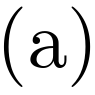
\includegraphics{figures/(a).png}

}

}

\end{minipage}%
%
\begin{minipage}[t]{0.01\linewidth}

{\centering 

~

}

\end{minipage}%
%
\begin{minipage}[t]{0.45\linewidth}

{\centering 

\raisebox{-\height}{

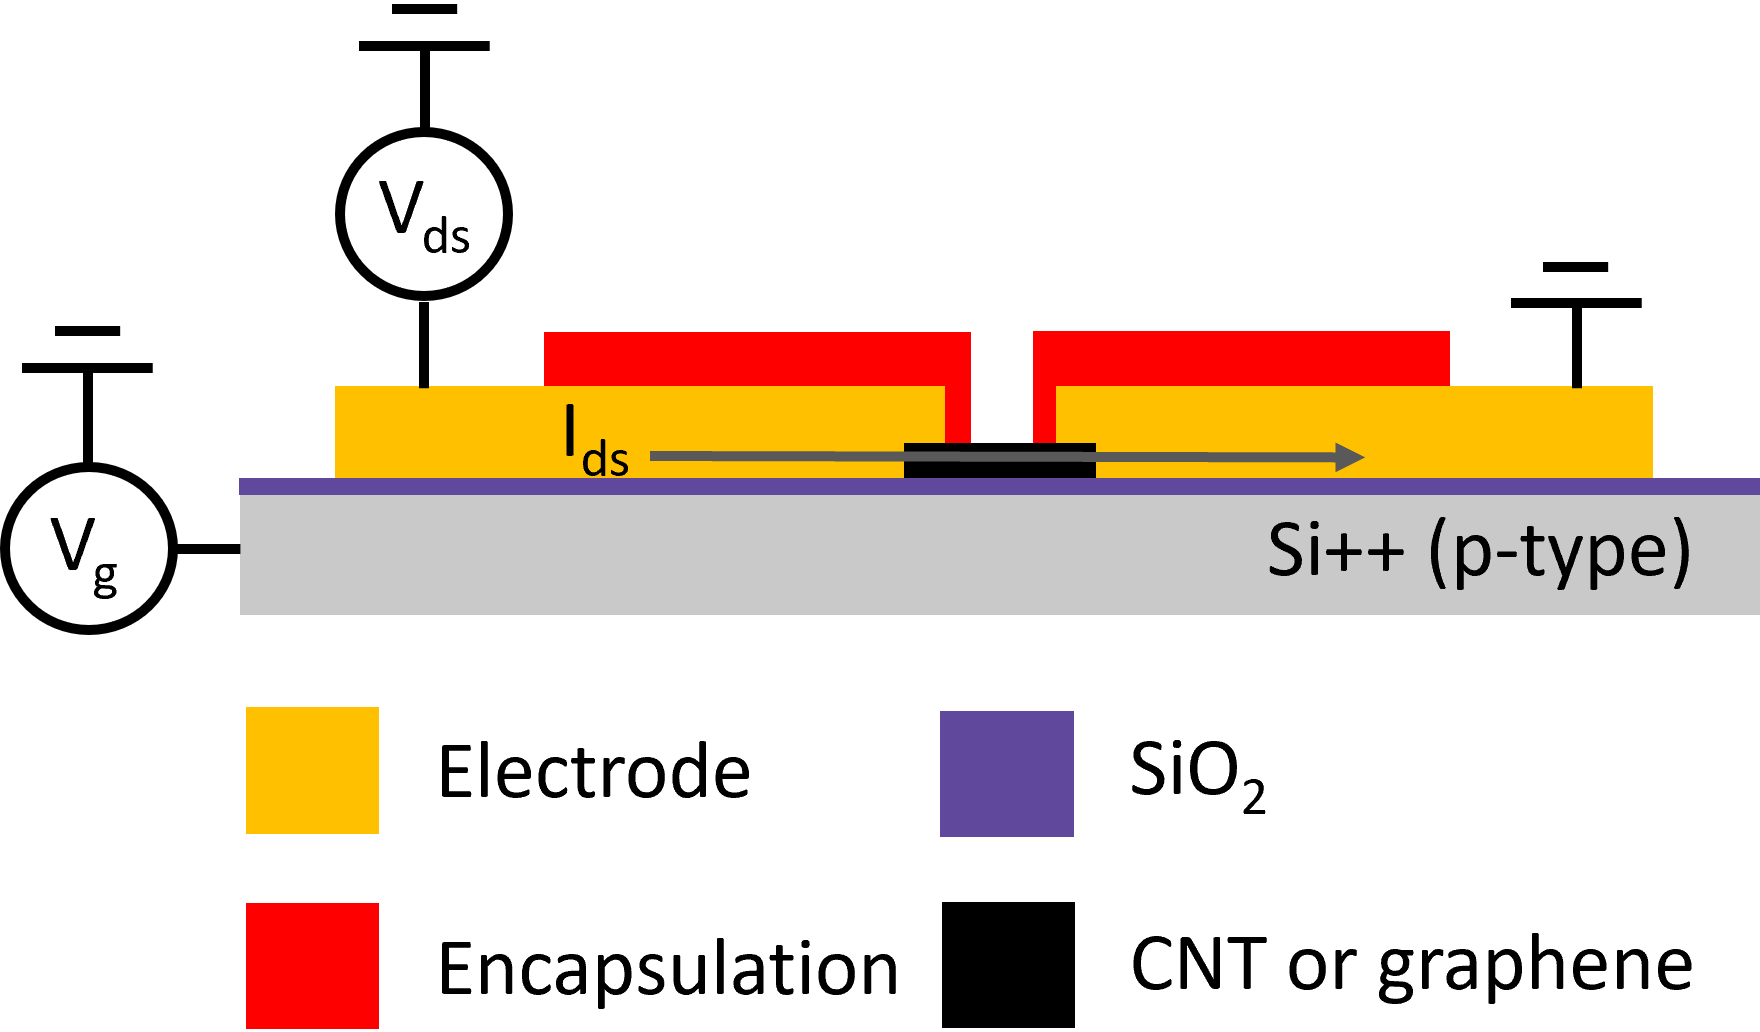
\includegraphics{figures/ch2/back-gate-schematic.png}

}

}

\end{minipage}%
%
\begin{minipage}[t]{0.01\linewidth}

{\centering 

~

}

\end{minipage}%
%
\begin{minipage}[t]{0.03\linewidth}

{\centering 

\raisebox{-\height}{

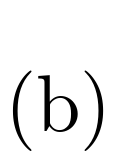
\includegraphics{figures/(b).png}

}

}

\end{minipage}%
%
\begin{minipage}[t]{0.01\linewidth}

{\centering 

~

}

\end{minipage}%
%
\begin{minipage}[t]{0.45\linewidth}

{\centering 

\raisebox{-\height}{

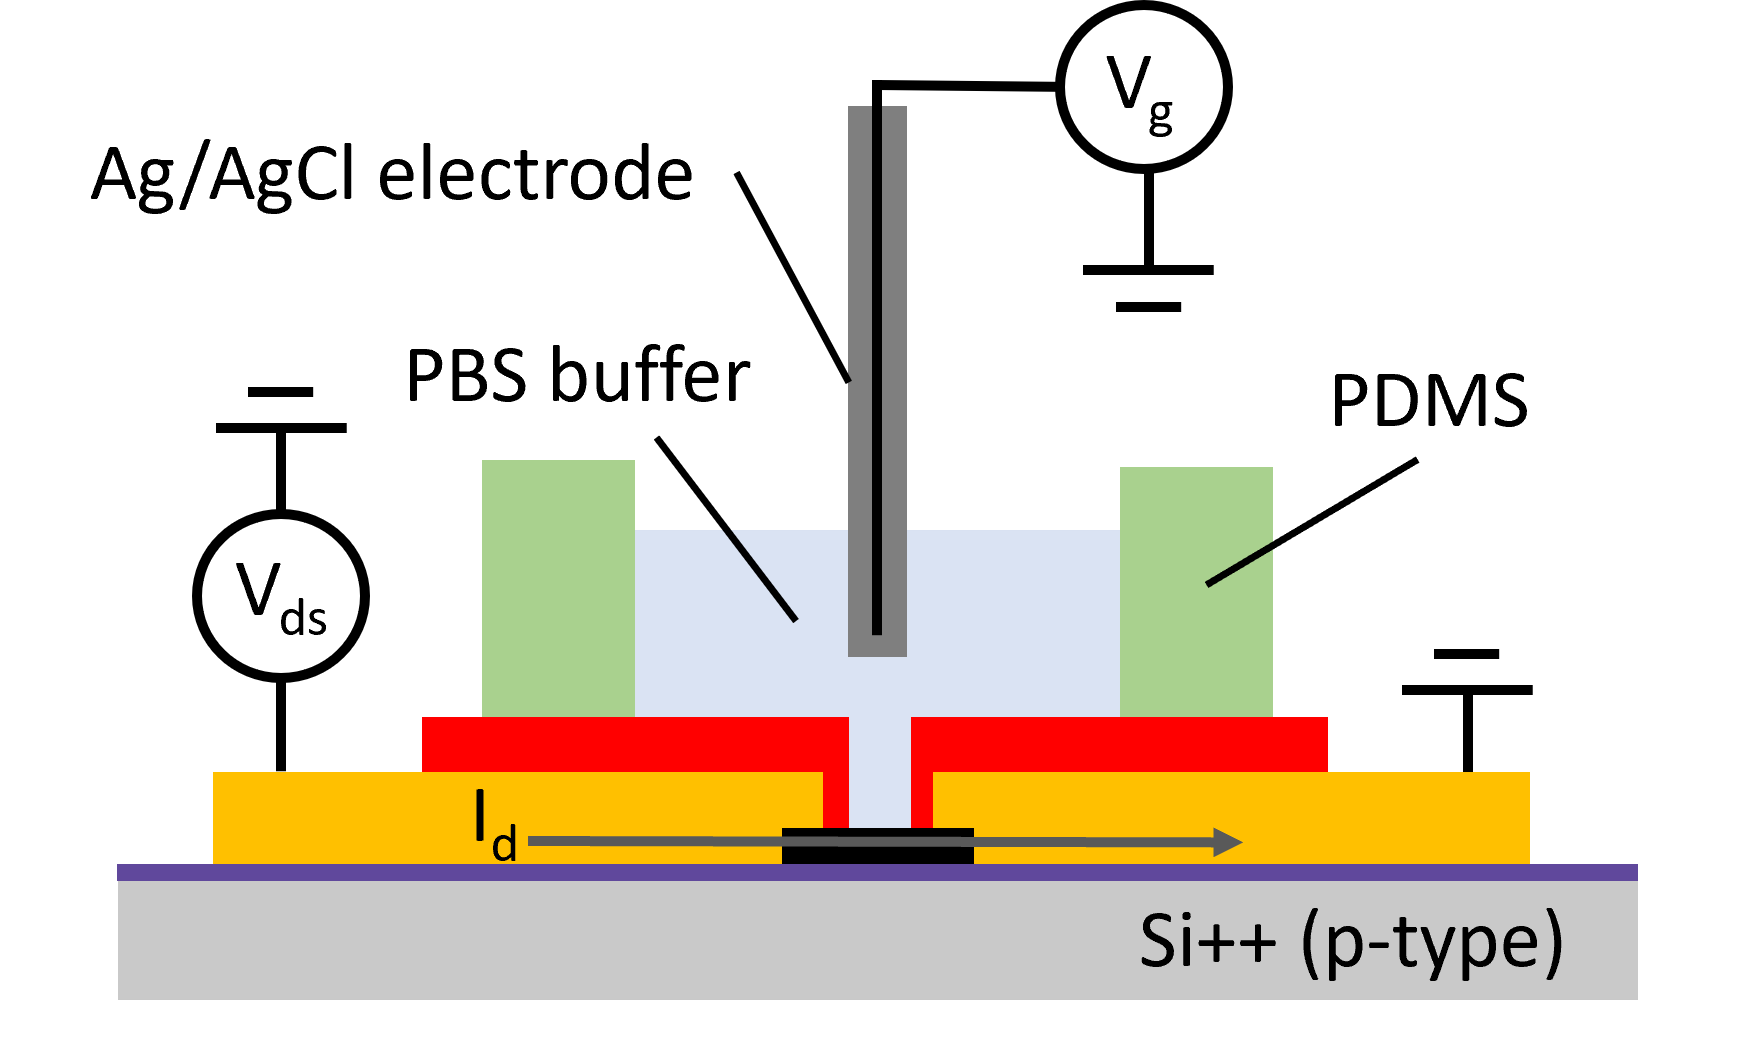
\includegraphics{figures/ch2/liquid-gate-schematic.png}

}

}

\end{minipage}%
%
\begin{minipage}[t]{0.01\linewidth}

{\centering 

~

}

\end{minipage}%

\caption{\label{fig-gating-schematics}Schematics (not to scale) showing
the side-view cross-section of a thin-film field-effect transistor in
both the (a) back-gated and (b) liquid-gated configuration. A graphene
monolayer or a carbon nanotube network is used as the transistor
thin-film. The drain electrode is the gold contact on the left side of
each figure, while the source electrode is the gold contact on the
right.}

\end{figure}

Two different voltages are used to adjust transistor operation. The
first is the `drain bias', \(V_{ds}\), between the drain and source
electrodes, and the second is the `gate bias', \(V_g\), applied between
the gate and source electrode. The value of \(V_g\) determines how
charge carriers flow under the influence of \(V_{ds}\) to produce a
drain-source current \(I_d\). The relative effect of changes in \(V_g\)
on source-drain current \(I_d\) is determined by gate capacitance. In
the general case, gate capacitance is a series combination of geometric
capacitance, \(C_{G}\), and the quantum capacitance of the channel
nanomaterial, \(C_{Q}\)
\autocite{Avouris2007,Cao2009,Heller2009a,Tran2016,Li2023}. Diameter and
separation of nanotubes also play a role in the case of carbon nanotube
networks \autocite{Rouhi2011a}. In an ambipolar transistor, a highly
negative \(V_g\) will give rise to hole conduction, and a highly
positive \(V_g\) will give rise to electron
conduction\autocite{Avouris2007,Yao2021,Li2023}. When
\(|V_{ds}| < |V_g| - |V_t|\) and the device is gated on, the device is
in the linear regime. In this regime, \(V_{ds}\) is directly
proportional to \(I_{d}\), similar to an Ohmic resistor. When
\(|V_{ds}| > |V_g| - |V_t|\) and the device is on, the device is in the
saturation regime, where the relationship between \(V_{ds}\) and
\(I_{d}\) becomes non-linear \autocite{Petti2016,Shkodra2021,Li2023}.

\hypertarget{liquid-gating-and-debye-length}{%
\subsubsection*{Liquid-Gating and Debye
Length}\label{liquid-gating-and-debye-length}}
\addcontentsline{toc}{subsubsection}{Liquid-Gating and Debye Length}

\begin{figure}

{\centering 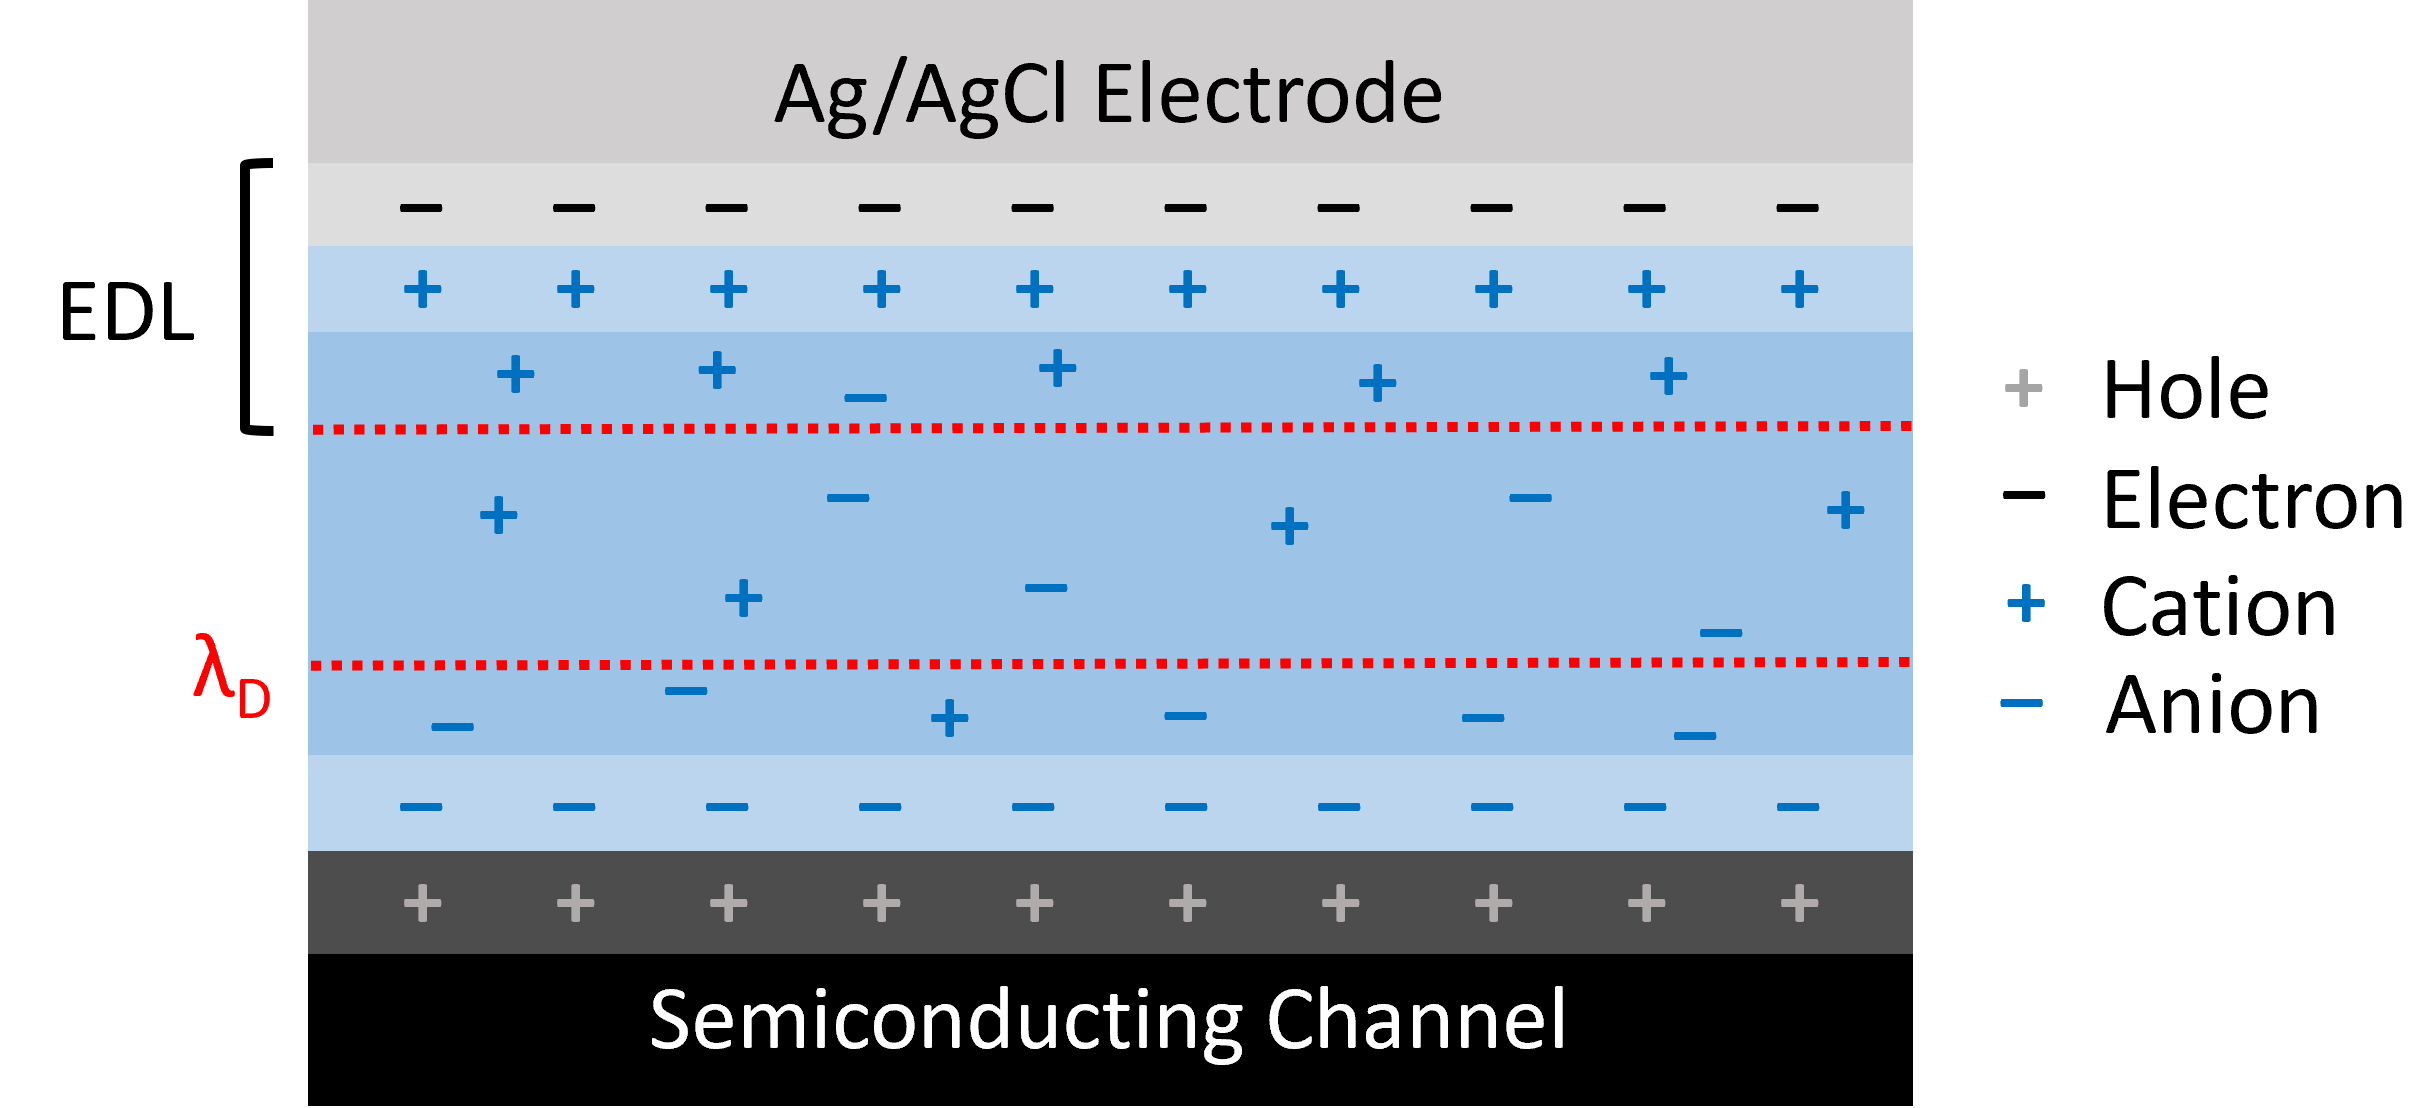
\includegraphics[width=0.7\textwidth,height=\textheight]{figures/ch2/Debye-length-schematic-alt.png}

}

\caption{\label{fig-Debye-length}A diagram of the formation of an
electric double layer (EDL) under an applied voltage between source and
liquid-gate electrodes, with a \(p\)-type semiconductor used for the
channel thin-film. Electric double layers are present at both the
gate-electrolyte interface and semiconductor-electrolyte interface.
Adapted from \autocite{Ohno2015,Shkodra2021,Tiwari2022}.}

\end{figure}

Understanding the ionic behaviour of the gate electrolyte used in a
liquid-gated device setup gives insight into the gating and sensing
behaviour of the setup. When a voltage is applied at the liquid-gate,
the charged ions in solution move to form two electric double layers,
one at the interface between the electrolyte and gate electrode, and one
at the interface between electrolyte and semiconducting channel, as
shown in Figure~\ref{fig-Debye-length}. The gate capacitance is a series
combination of the capacitance of each EDL in series with quantum
capacitance \(C_{Q}\) \autocite{Heller2010,Shkodra2021}. The
Gouy-Chapman-Stern model splits the EDL into two distinct regions, the
first being a compact layer of ions, the Stern layer, and the second
being a more diffuse layer, the Gouy-Chapman layer
\autocite{Tiwari2022}. The surface potential of the solid-electrolyte
interface exponentially decreases across the diffuse region of the
double-layer; the characteristic length of this potential screening is
known as Debye length, \(\lambda_D\). The typical electrolyte Debye
length is on a nanometer scale, therefore the bulk electrolyte acts as
an insulator, similar to the silicon dioxide dielectric in the
back-gated configuration. The Stern layer capacitance is inversely
proportional to the Debye length, and therefore decreased \(\lambda_D\)
corresponds to increased gate capacitance
\autocite{Heller2010,Ohno2015,Shkodra2021,Yao2021}.

\begin{equation}\protect\hypertarget{eq-debye-length}{}{
\lambda_D = \sqrt{\frac{\epsilon_0\epsilon_rk_bT}{2N_Aq^2I}}
}\label{eq-debye-length}\end{equation}

The equation for Debye length \(\lambda_D\) in an electrolyte solution
is given by Equation~\ref{eq-debye-length}, where \(\epsilon_0\) is
vacuum permittivity, \(\epsilon_r\) is the relative permittivity of the
electrolyte, \(\k_B\) is the Boltzmann constant, \(T\) is absolute
temperature in K, \(N_A\) is the Avogadro number, \(q\) is the
elementary charge and \(I\) is ionic strength in mmol L\(^{-1}\). When
temperature is kept constant, \(\lambda_D\) only depends on the ionic
strength of the electrolyte and not on any attributes of the gate
electrode or channel. Successive dilutions of a particular electrolyte
will increase the Debye length: for \(1 \times\) PBS, \(\lambda_D\) is
0.7 nm, for \(0.1 \times\) PBS, \(\lambda_D\) is 2.3 nm, for
\(0.01 \times\) PBS \(\lambda_D\) is 7.3 nm and so on. This means gate
capacitance is directly dependent on the electrolyte used and its
concentration. A \(1 \times\) PBS electrolyte gives a gate capacitance
several orders of magnitude larger than that of a silicon oxide
back-gate. A larger capacitance significantly increases the effect of
electrostatic gating on the channel current, often described as
increased electrostatic coupling between gate and channel. A
liquid-gated device with low Debye length will therefore be highly
sensitive to electrostatic changes across a small voltage range
\autocite{Heller2010,Wang2010,Ohno2015,Shkodra2021,Yao2021}.

However, a decreased Debye length also has disadvantages for sensing.
Electrostatic potentials outside of the electrolyte-channel electrical
double layer are effectively screened from the channel. Electrical
double layers will also form around charged receptors within the
solution. The combined screening effect means signals due to potential
changes in charged biomolecules within the bulk electrolyte will have no
effect on gating of the channel, and therefore no effect on \(I_d\).
Interactions between the analyte and any receptor element must therefore
occur within the Debye length, and so a tradeoff exists between channel
sensitivity and the size of the sensitive region above the channel. Many
medium or large proteins will require a relatively dilute electrolyte
for analyte capture to be detected by the channel, which may not reflect
the intended environment for biosensor application
\autocite{Stern2007,Piccinini2018,Shkodra2021}. Other approaches to
increasing Debye length without reducing device sensitivity have
therefore also been trialled. One approach involves attaching a layer of
polyethylene glycol polymer (PEG) to the channel, limiting the approach
of counterions. This increases Debye length at the electrolyte-channel
interface while preserving the capacitance of the electrolyte-gate
interface, keeping device sensitivity relatively high
\autocite{Gao2016,Kesler2020,Albarghouthi2022}.

\hypertarget{electrical-characterisation}{%
\subsection{Electrical
Characterisation}\label{electrical-characterisation}}

Both carbon nanotube field effect transistors and graphene field-effect
transistors are naturally ambipolar. Applying a gate voltage \(V_g\) to
the gate of an ambipolar thin-film transistor influences the amount and
type of available charge carriers for conduction
\autocite{Avouris2007,Tran2016,Heller2009a}. The current-voltage plots
for a given transistor are known as the `characteristic curves' of the
transistor. The plot of \(I_d\) against \(V_g\) at constant \(V_{ds}\)
is known as the `transfer' characteristic curve at that source-drain
voltage, while the I-V curve of \(I_d\) against \(V_{ds}\) at constant
\(V_g\) is known as the `source-drain' or `output' characteristic curve
at that gate voltage \autocite{Petti2016,Shkodra2021}. The transfer
characteristics are governed by the gate capacitance, as discussed in
Section~\ref{sec-gating}. Both back-gated and liquid-gated transfer
characteristics from ambipolar thin-film transistors are shown in
Figure~\ref{fig-gating-transfer}. Taking regular transfer measurements
of a graphene or carbon nanotube device is not only useful in building a
complete picture of device behaviour, but also may help to ensure
devices are kept highly sensitive to electrostatic gating effects
through redistributing charge in the channel \autocite{Noyce2019}.

A variety of quantitative parameters can be extracted from the transfer
characteristics of a thin-film transistor. A quantitative summary of a
range of TFT parameters can be found in the thin-film transistor study
by Petti \emph{et al.} \autocite{Petti2016}. The parameters of
particular interest here are transconductance, on-off ratio, threshold
voltage and subthreshold swing. Transconductance and on-off ratio are
discussed below, while threshold voltage and subthreshold swing are
discussed for the carbon nanotube network case specifically in
Section~\ref{sec-electrical-characterisation-CNT}. Other behaviours
observed when measuring currents present in a thin-film device are also
discussed below, including source-gate leakage current and the
hysteresis and real-time signal drift of source-drain current.

\begin{figure}

\begin{minipage}[t]{0.03\linewidth}

{\centering 

\raisebox{-\height}{

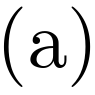
\includegraphics{figures/(a).png}

}

}

\end{minipage}%
%
\begin{minipage}[t]{0.01\linewidth}

{\centering 

~

}

\end{minipage}%
%
\begin{minipage}[t]{0.45\linewidth}

{\centering 

\raisebox{-\height}{

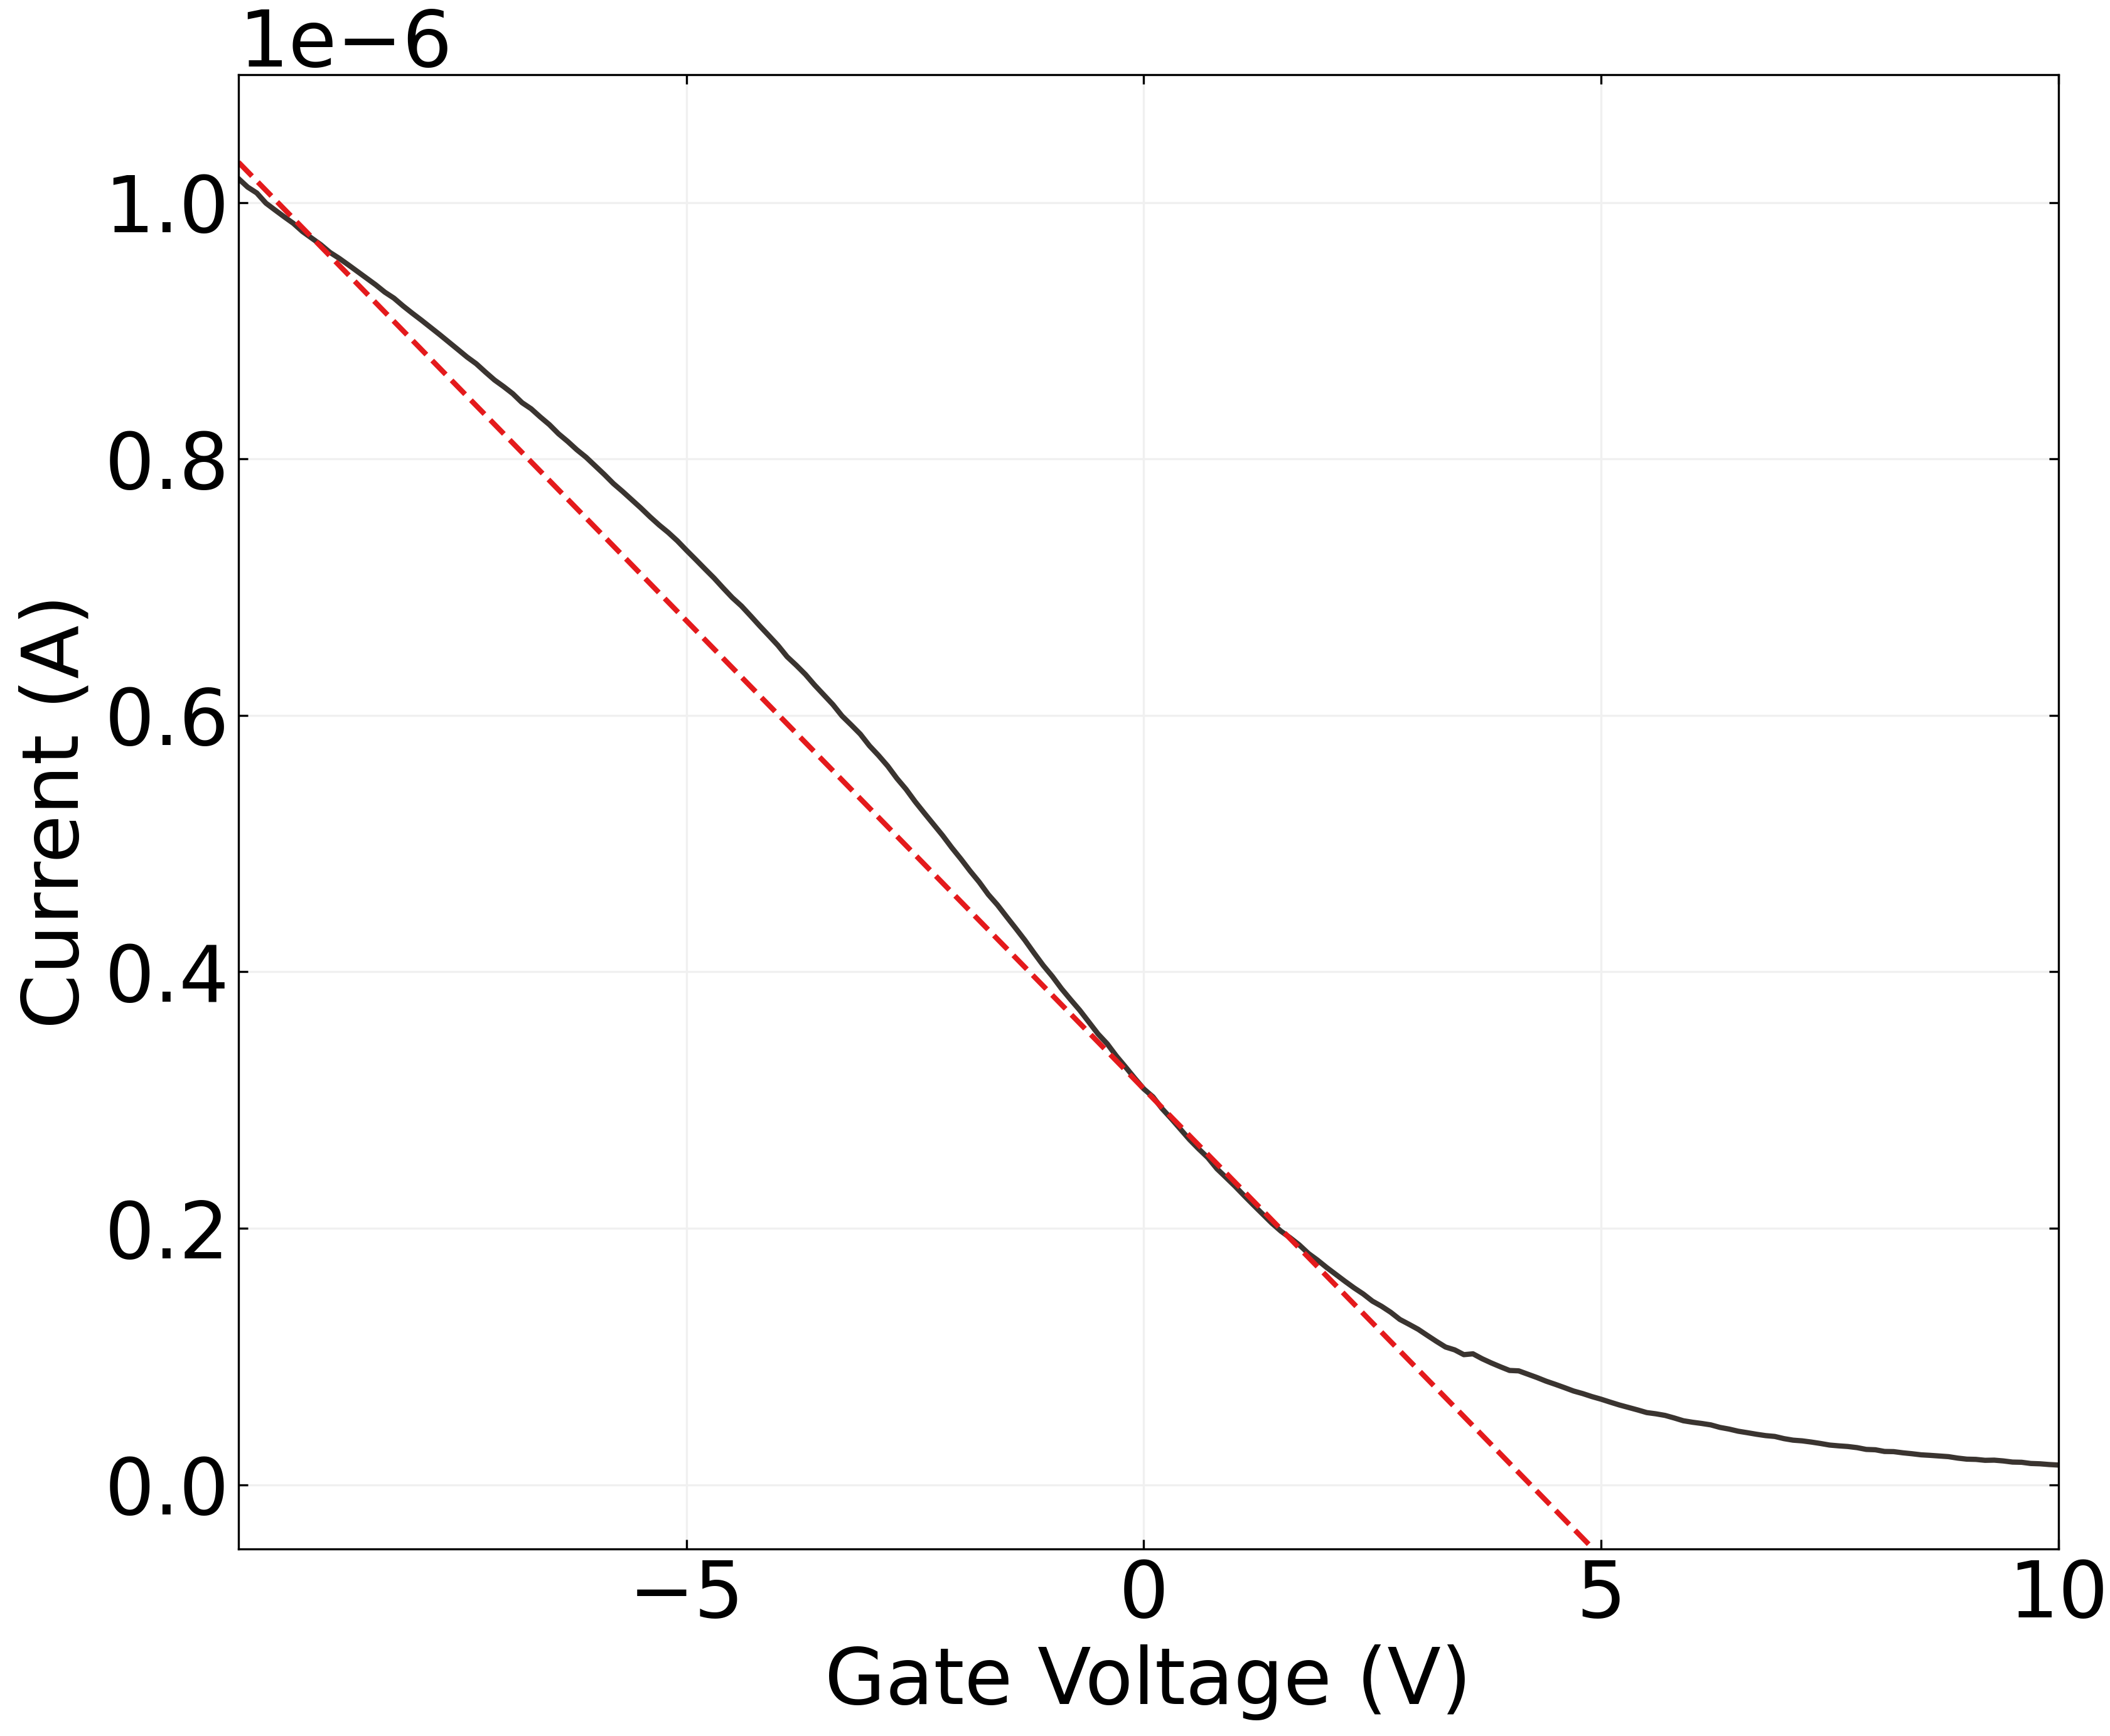
\includegraphics{figures/ch2/Q5C10ch5transconductance.png}

}

}

\end{minipage}%
%
\begin{minipage}[t]{0.01\linewidth}

{\centering 

~

}

\end{minipage}%
%
\begin{minipage}[t]{0.03\linewidth}

{\centering 

\raisebox{-\height}{

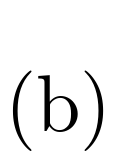
\includegraphics{figures/(b).png}

}

}

\end{minipage}%
%
\begin{minipage}[t]{0.01\linewidth}

{\centering 

~

}

\end{minipage}%
%
\begin{minipage}[t]{0.45\linewidth}

{\centering 

\raisebox{-\height}{

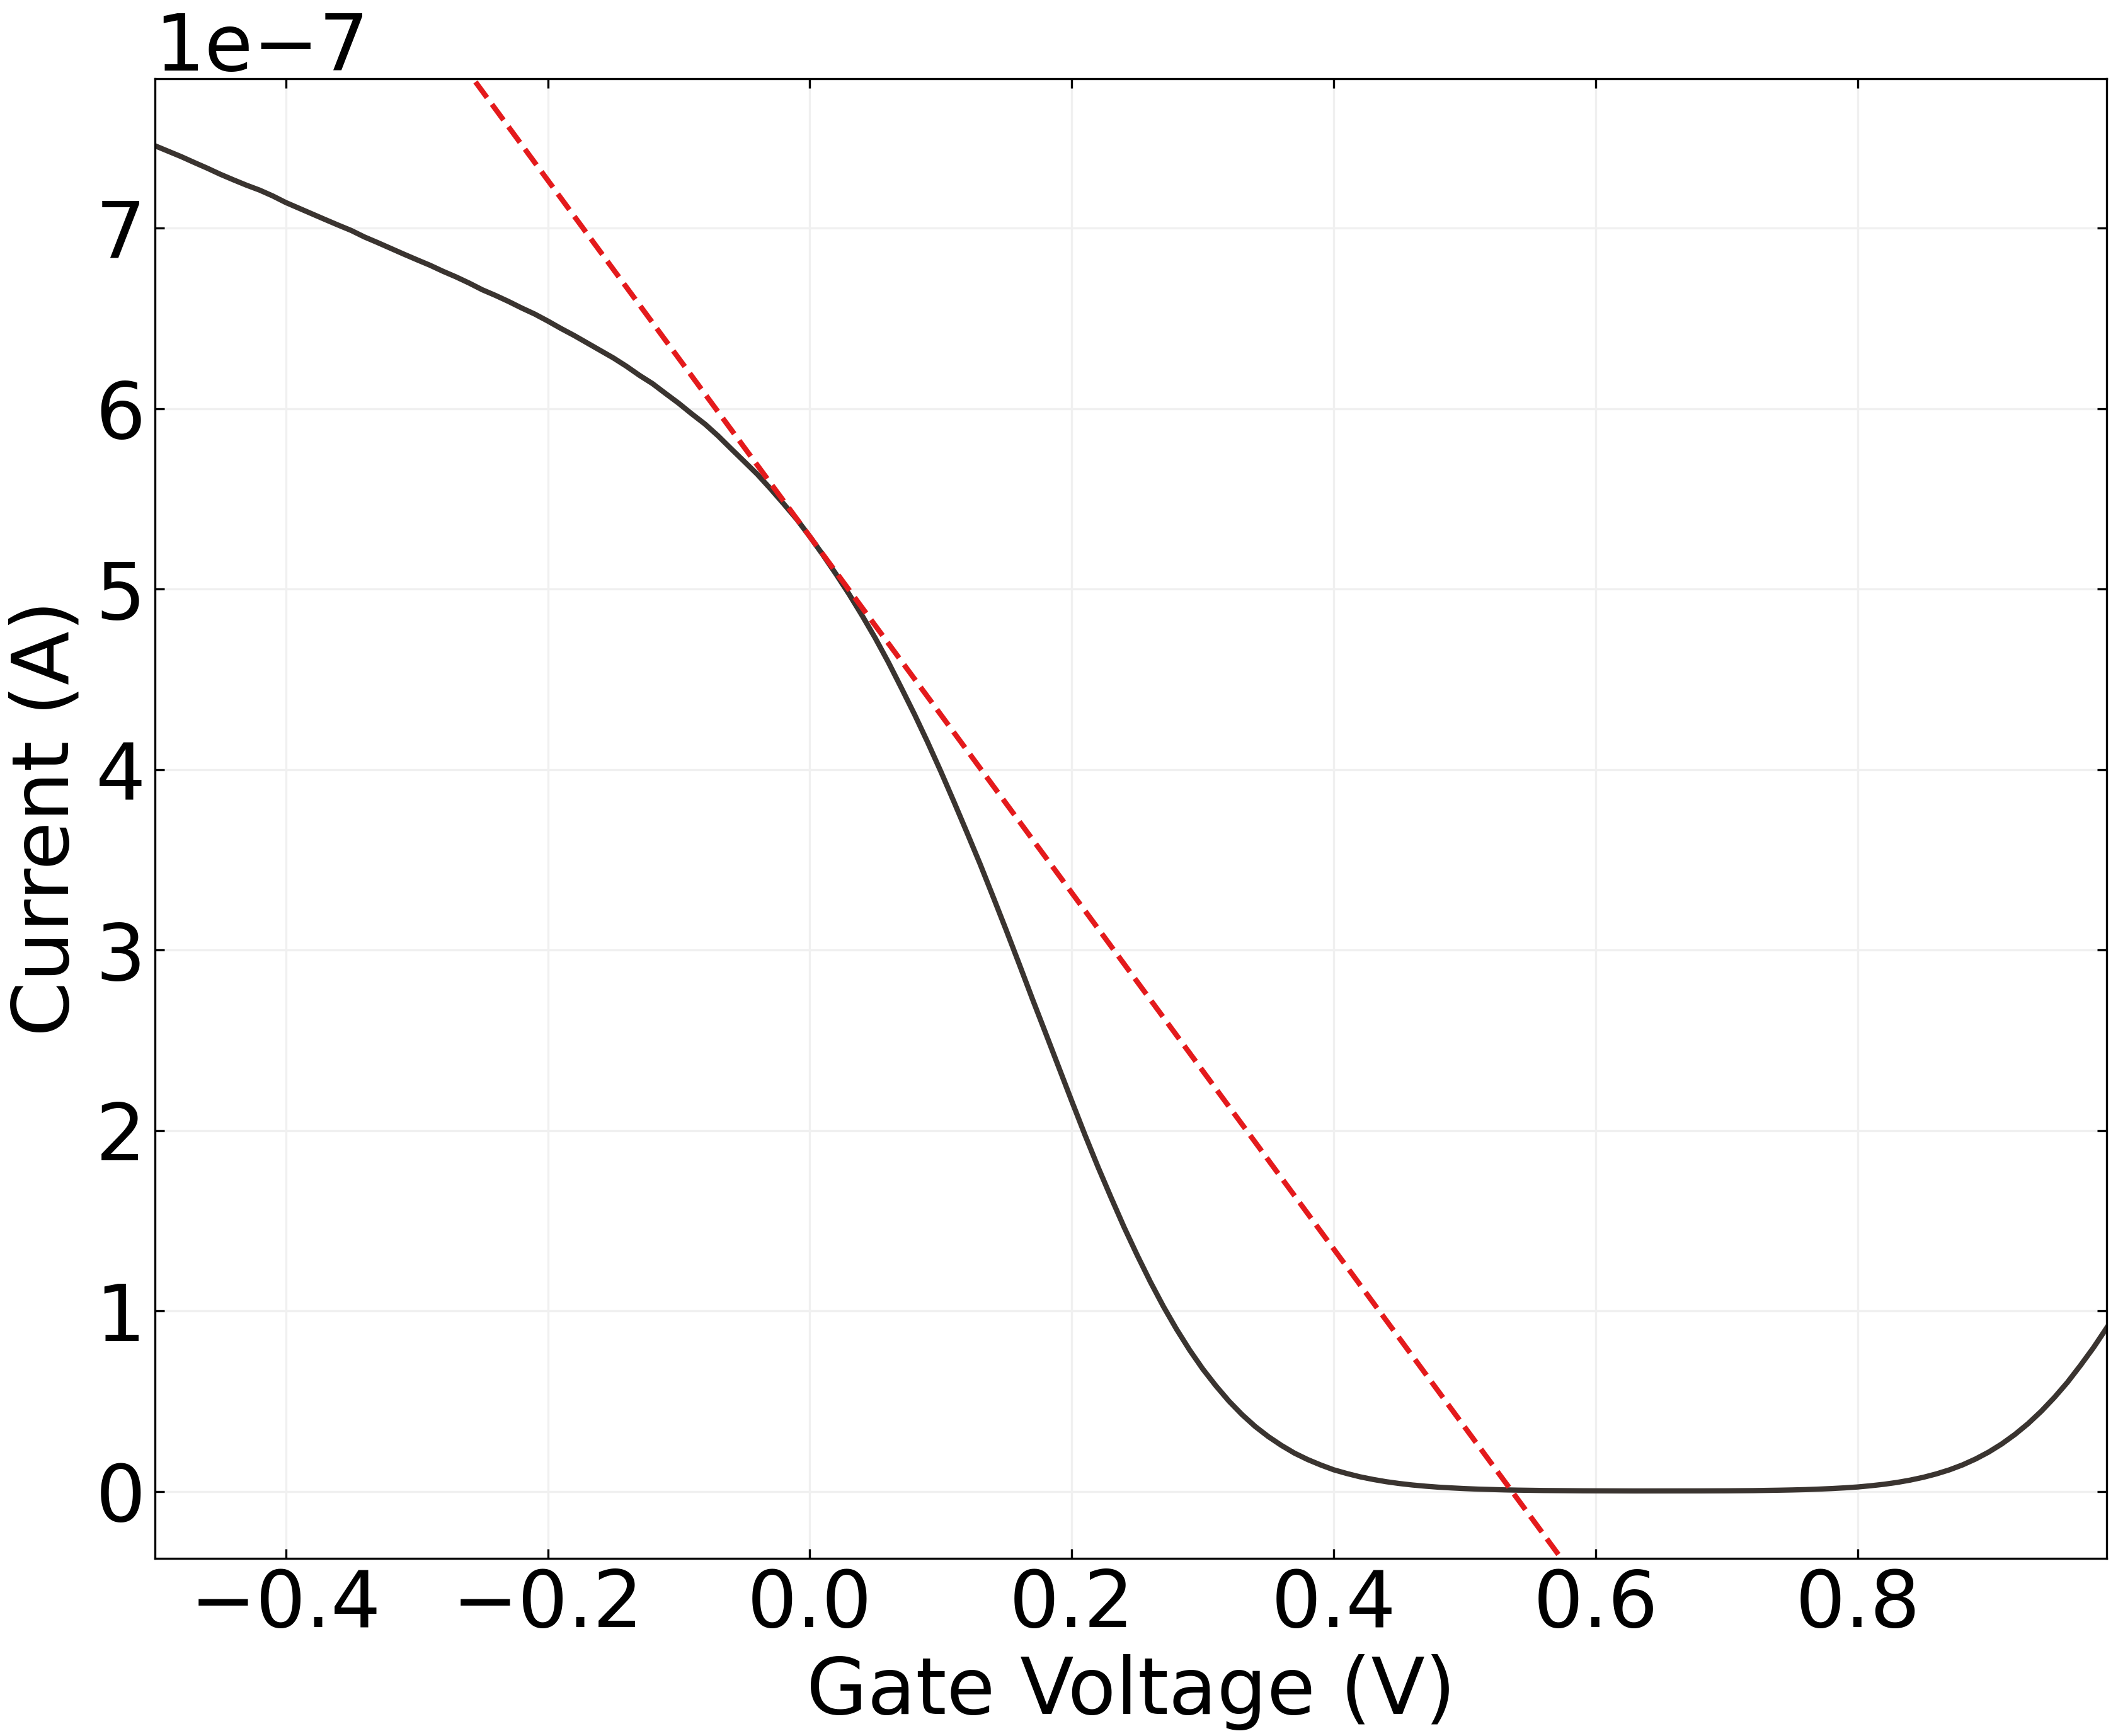
\includegraphics{figures/ch2/NTQ31C5ch1transconductance.png}

}

}

\end{minipage}%
%
\begin{minipage}[t]{0.01\linewidth}

{\centering 

~

}

\end{minipage}%
\newline
\begin{minipage}[t]{0.03\linewidth}

{\centering 

\raisebox{-\height}{

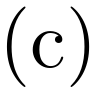
\includegraphics{figures/(c).png}

}

}

\end{minipage}%
%
\begin{minipage}[t]{0.01\linewidth}

{\centering 

~

}

\end{minipage}%
%
\begin{minipage}[t]{0.45\linewidth}

{\centering 

\raisebox{-\height}{

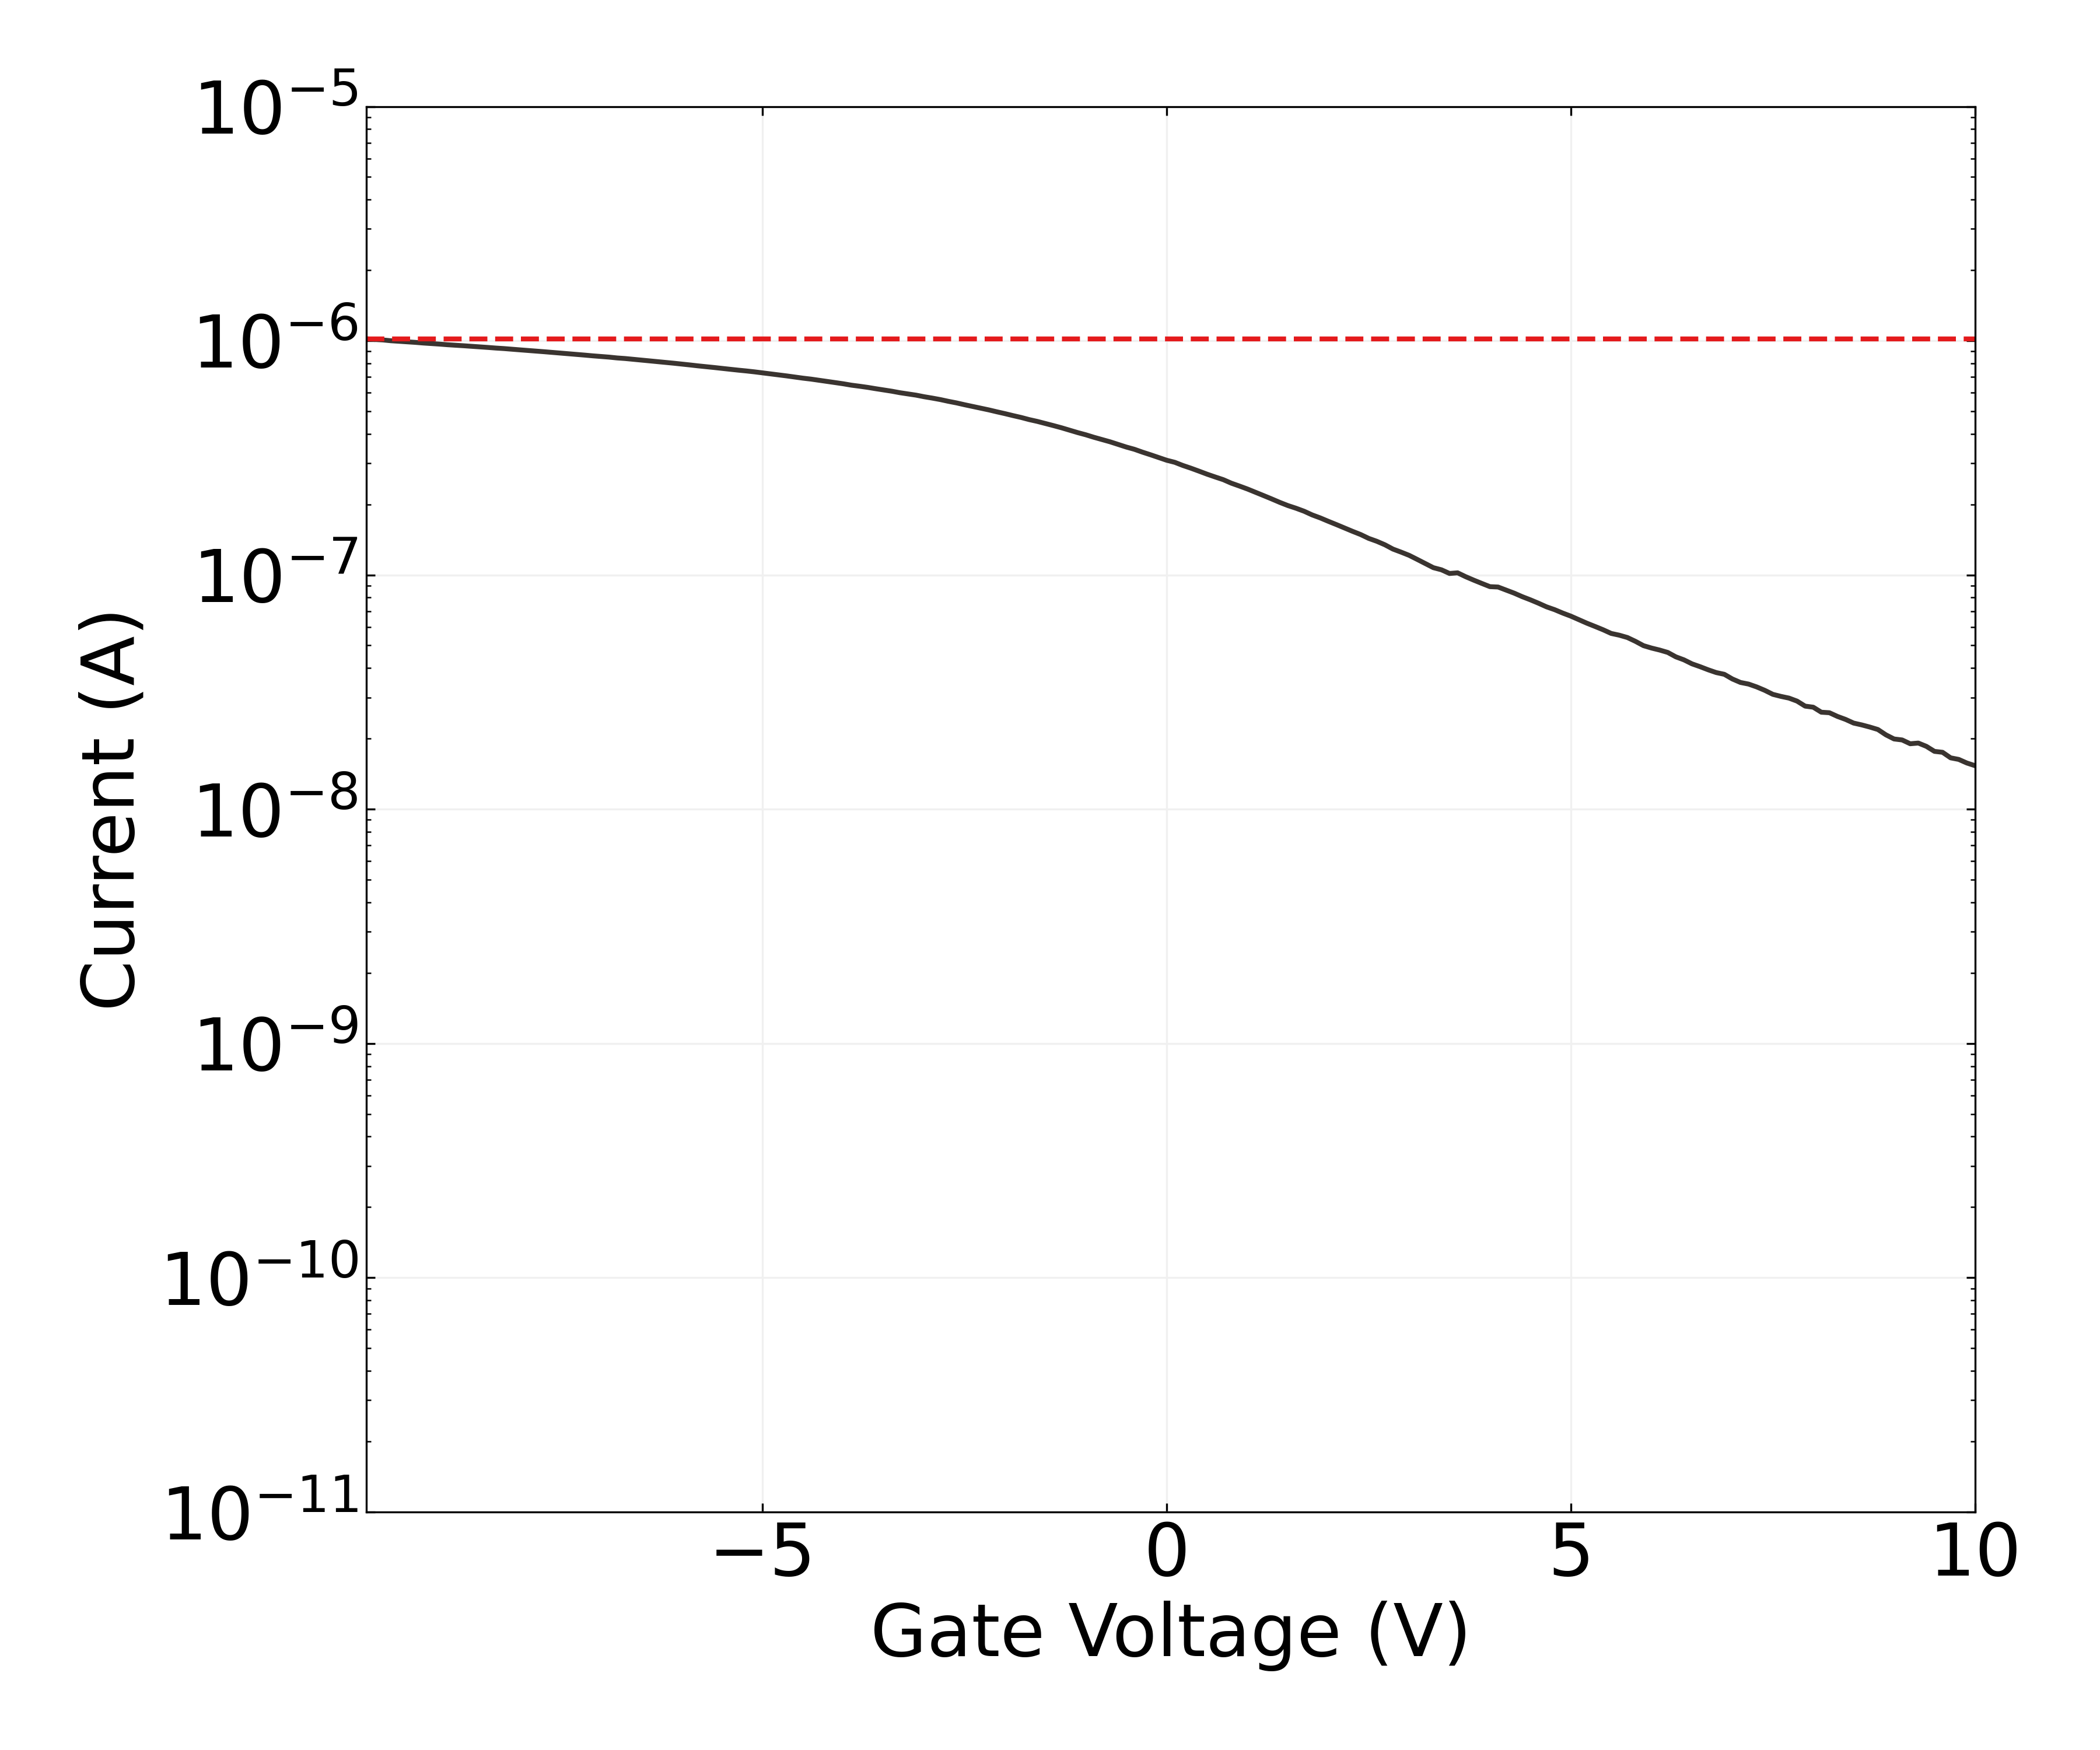
\includegraphics{figures/ch2/Q5C10ch5on_current.png}

}

}

\end{minipage}%
%
\begin{minipage}[t]{0.01\linewidth}

{\centering 

~

}

\end{minipage}%
%
\begin{minipage}[t]{0.03\linewidth}

{\centering 

\raisebox{-\height}{

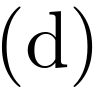
\includegraphics{figures/(d).png}

}

}

\end{minipage}%
%
\begin{minipage}[t]{0.01\linewidth}

{\centering 

~

}

\end{minipage}%
%
\begin{minipage}[t]{0.45\linewidth}

{\centering 

\raisebox{-\height}{

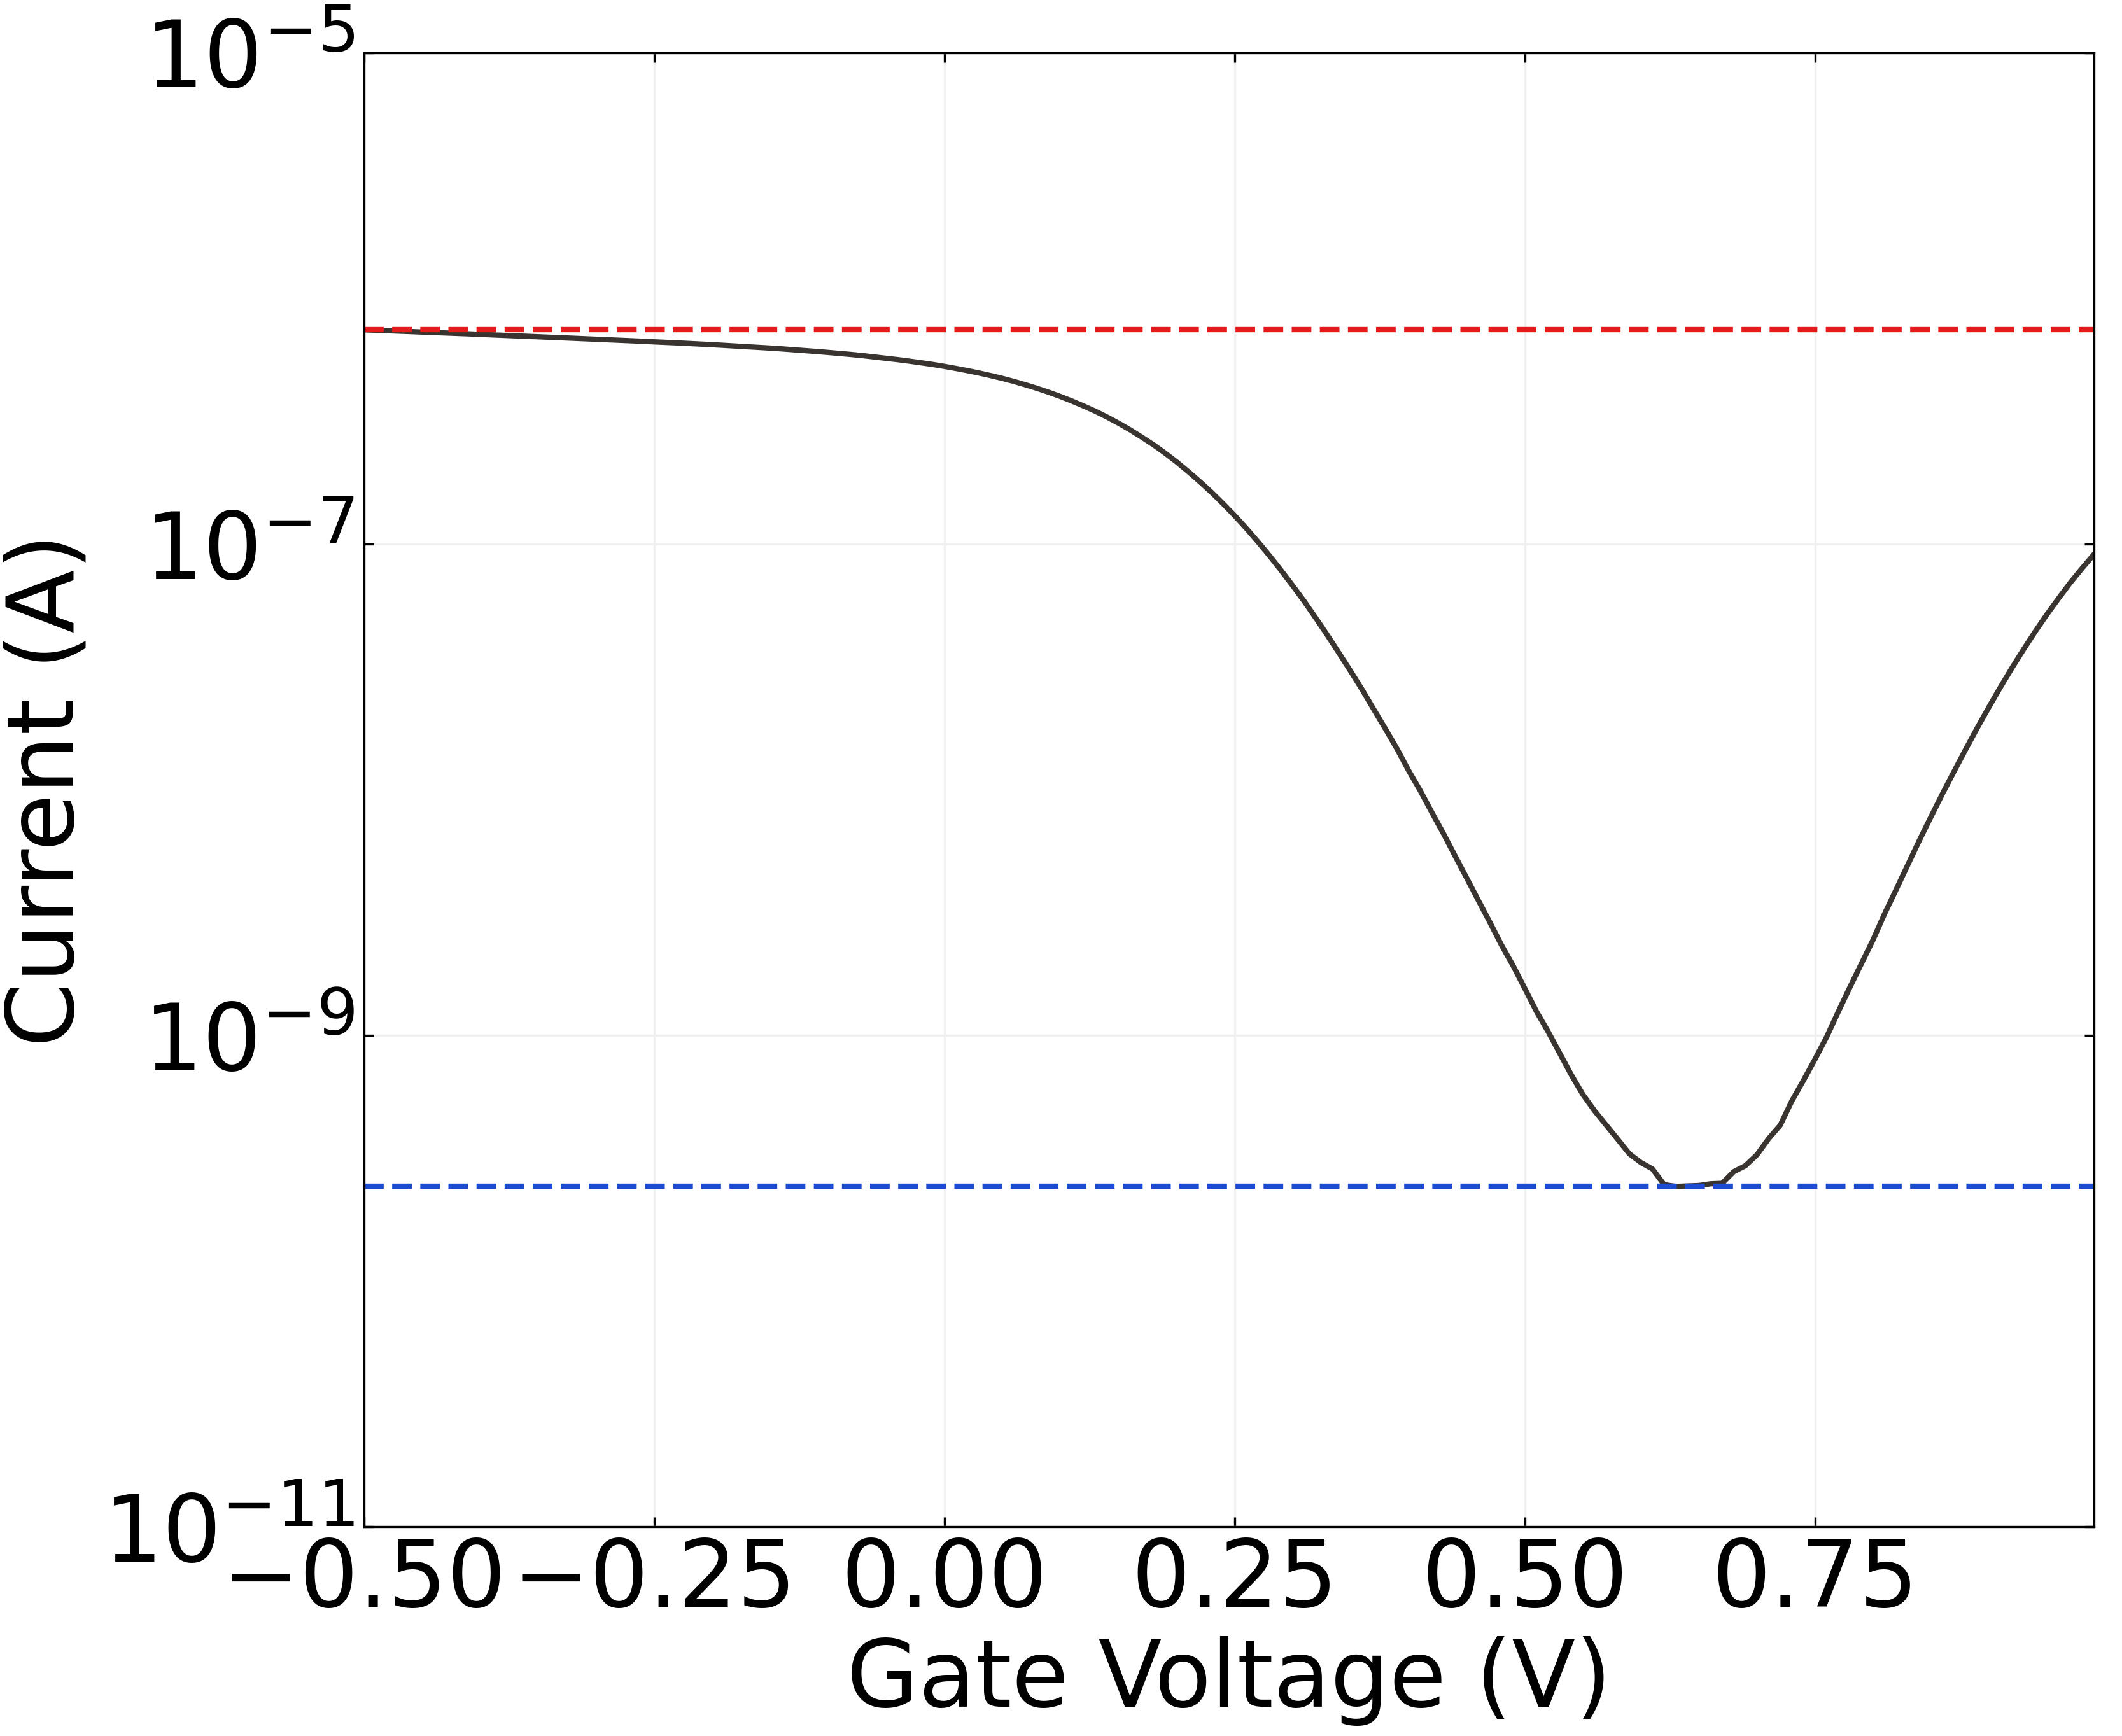
\includegraphics{figures/ch2/NTQ31C5ch1on_off_current.png}

}

}

\end{minipage}%
%
\begin{minipage}[t]{0.01\linewidth}

{\centering 

~

}

\end{minipage}%

\caption{\label{fig-gating-transfer}Examples of field-effect transistor
transfer characteristics taken at \(V_{ds}\) = 100 mV from two different
device channels. A linear scale is used in (a) and (b), while a
logarithmic scale is used in (c) and (d). The curves in (a) and (c) are
from backgated channels, while the curves in (b) and (d) are from
liquid-gated channels. The linear fit with gradient corresponding to
transconductance at \(V_g\) = 0 V is shown in (a) and (b) with a dotted
red line. The ``on'' current in (c) and (d) is shown with a red
horizontal line, while the ``off'' current in (d) is shown with a blue
horizontal line.}

\end{figure}

\hypertarget{transconductance}{%
\subsubsection*{Transconductance}\label{transconductance}}
\addcontentsline{toc}{subsubsection}{Transconductance}

In the linear regime, transconductance at a specific gate voltage is
given by \(g_m = |dI_{d}/dV_g|\). Transconductance indicates how
responsive the device is to electrostatic gating at a given gate
voltage. In other words, when \(g_m\) is large, small changes in \(V_g\)
can significantly modulate channel current \(I_d\), which is useful for
sensing \autocite{Heller2009a,Ohno2015}. Transconductance at a given
gate voltage is also proportional to the mobility (movement) of charge
carriers in the device channel, and therefore depends on the scattering
properties of the material \autocite{Rouhi2010,Petti2016,Li2023}. The
transconductance at a specific gate voltage can be found from performing
a linear fit in a small region around that voltage on the transfer
curve. Linear fits for transconductance at \(V_g = 0\) V are shown for a
back-gated device in Figure~\ref{fig-gating-transfer} (a), and a
liquid-gated device in Figure~\ref{fig-gating-transfer} (b), which give
values of \(g_m\) = 0.05 µS and \(g_m\) = 1 µS respectively. The
difference of several orders of magnitude between back-gated and
liquid-gated transconductance corresponds to the difference of several
orders of magnitude between back and liquid-gated gate capacitance
\autocite{Tran2016,Shkodra2021}. Improved transconductance is therefore
a significant advantage of the use of the liquid-gate.

\hypertarget{on-off-ratio}{%
\subsubsection*{On-off Ratio}\label{on-off-ratio}}
\addcontentsline{toc}{subsubsection}{On-off Ratio}

Another important attribute of the transfer characteristic curve for all
thin-film FETs is the on-off current ratio. On-off current ratio is the
ratio of the current through a device when gated fully `off' with a
positive voltage, \(I_{off}\), to the current through the device when
gated fully `on' with a negative voltage, \(I_{on}\). The off current in
an ambipolar FET can be defined as the minimum current during the
transfer sweep, where the majority carrier transitions from being holes
to electrons or \emph{vice versa} \autocite{Petti2016,Zheng2017}. For
example, for the channel shown in Figure~\ref{fig-gating-transfer} (b),
\(I_{on} = 741.5\) nA and \(I_{off} = 0.2\) nA. Therefore, the on-off
ratio \(I_{on}/I_{off}\) is \(\sim\) 3000. In contrast, even when 10 V
is applied, the backgated device shown in
Figure~\ref{fig-gating-transfer} (a) is never gated fully off. Being
able to traverse both on and off regimes over a limited voltage interval
is another advantage of the liquid-gated configuration. Having a low off
current is desirable as it corresponds to low power consumption by the
transistor \autocite{Rouhi2010}. Overall, on-off ratio of a device is a
useful figure of merit for switching which is relatively simple to both
find and present.

\hypertarget{gate-leakage}{%
\subsubsection*{Gate Leakage}\label{gate-leakage}}
\addcontentsline{toc}{subsubsection}{Gate Leakage}

Application of higher voltages to the gate in both the liquid-gate and
back-gate cases can result in significant leakage currents through the
gate. These currents mean that the insulating layer at the gate
producing the capacitive effect no longer acts as an insulator,
adversely affecting transistor behaviour and contributing to sensor
drift that may be mistaken for signal responses to
analyte\autocite{Noyce2019,Shkodra2021,Albarghouthi2022}. In the case of
back-gated devices, gate leakage occurs due to conduction through the
oxide dielectric. If the gate voltage produces an electric field
exceeding the dielectric strength of the oxide, dielectric breakdown can
occur, where the oxide layer no longer acts as an insulator. Breakdown
results from voltage-induced oxygen vacancies in the SiO\(_2\) lattice
forming a conductive path through the insulator \autocite{Padovani2017}.
In the liquid-gated case, the choice of electrolyte determines the
appropriate voltage range for electrical characterisation, since
excessive voltages will drive electrolysis and induce redox reactions.
For water-based electrolytes, gate voltages must be kept within the
\(\pm\) 1 V range \autocite{Wang2010,Ohno2015,Shkodra2021}. In normal
operation, gate current should appear negligible on a linear scale for
both the back-gated and liquid-gated cases, as shown in
Figure~\ref{fig-gating-hysteresis}.

\begin{figure}

\begin{minipage}[t]{0.03\linewidth}

{\centering 

\raisebox{-\height}{

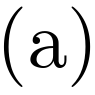
\includegraphics{figures/(a).png}

}

}

\end{minipage}%
%
\begin{minipage}[t]{0.01\linewidth}

{\centering 

~

}

\end{minipage}%
%
\begin{minipage}[t]{0.45\linewidth}

{\centering 

\raisebox{-\height}{

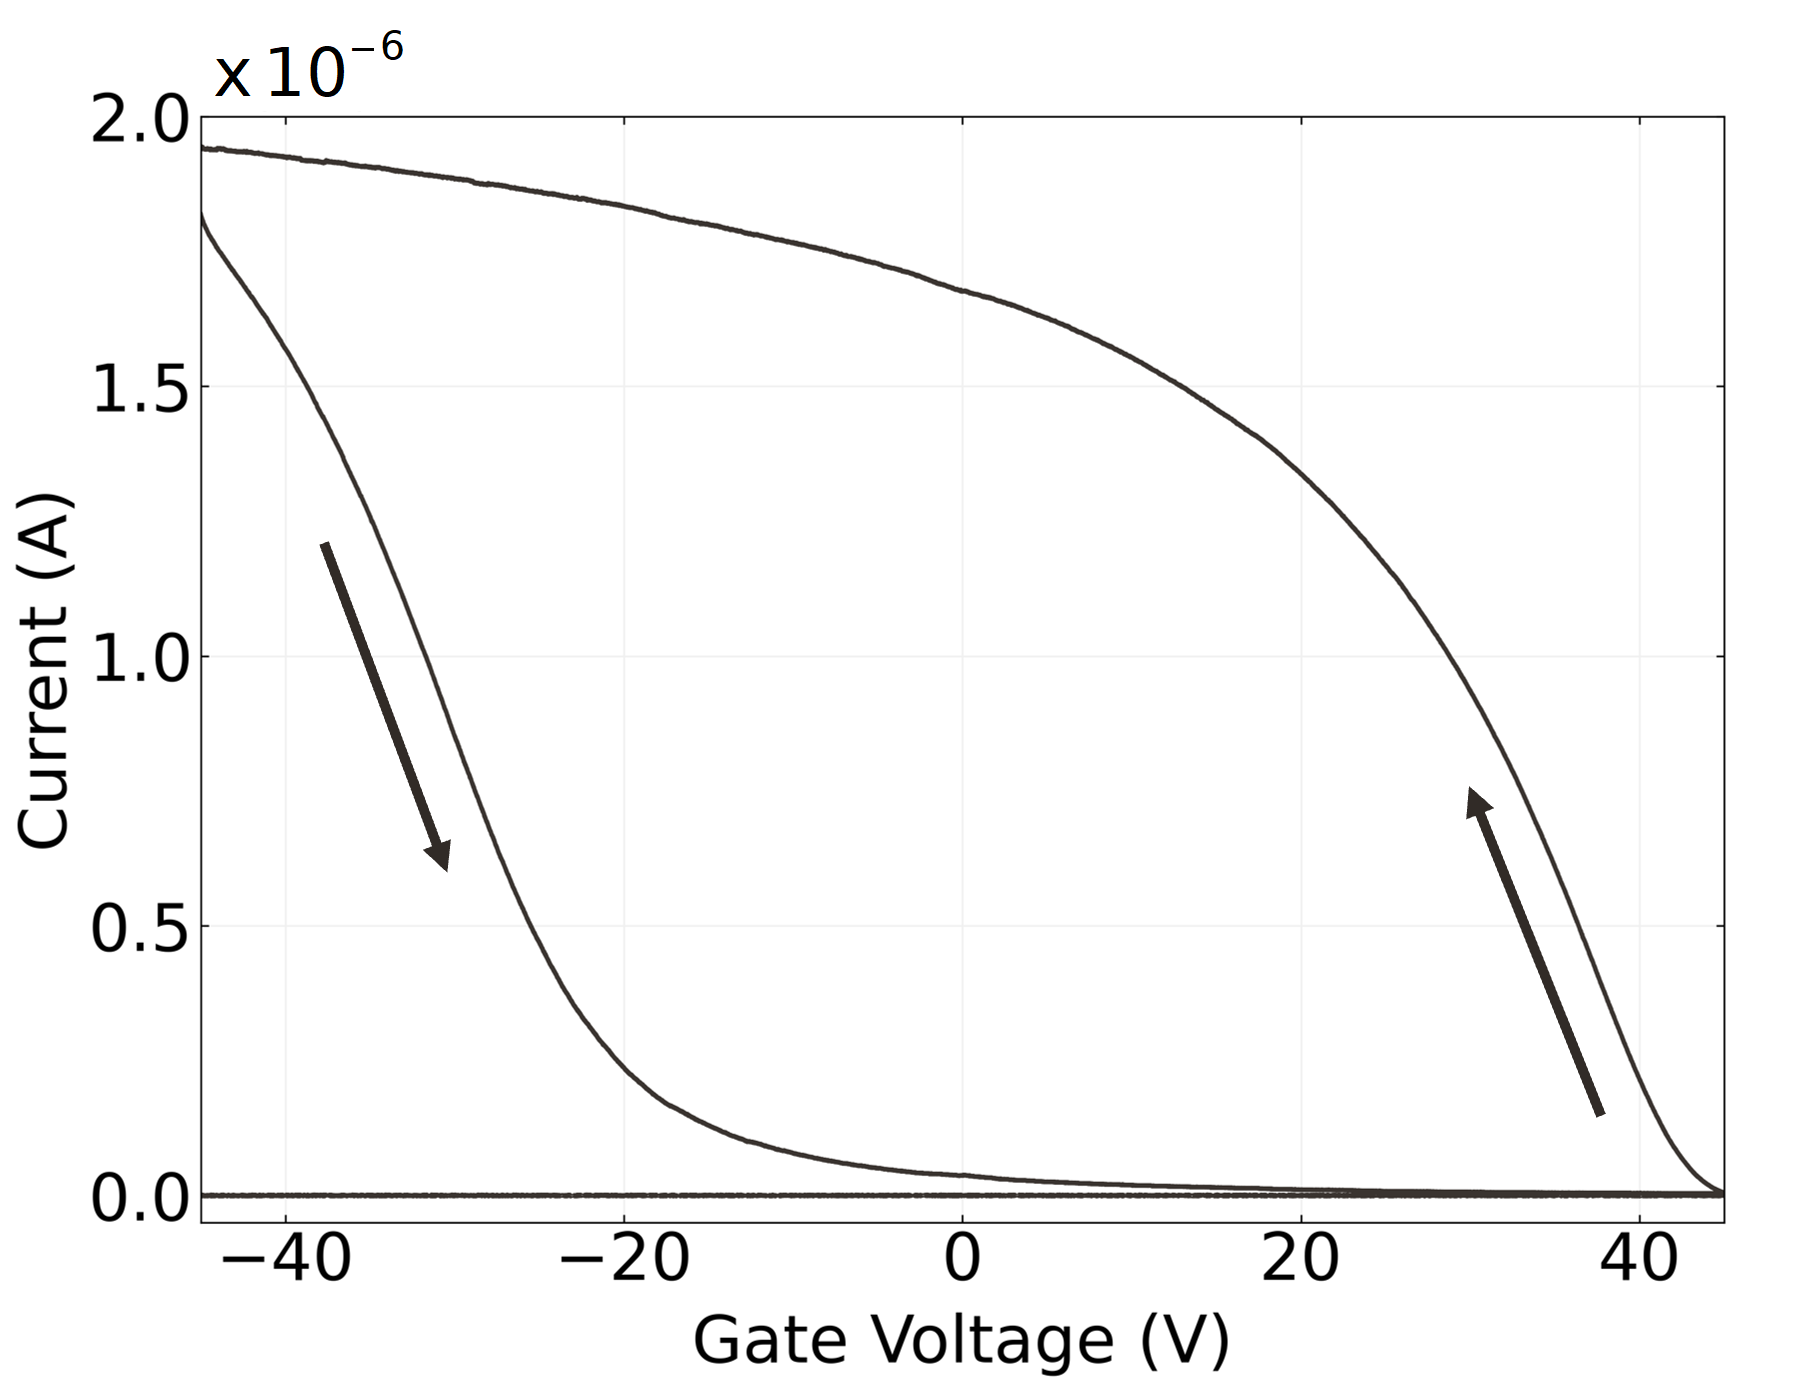
\includegraphics{figures/ch2/Q5C10_hysteresis.png}

}

}

\end{minipage}%
%
\begin{minipage}[t]{0.01\linewidth}

{\centering 

~

}

\end{minipage}%
%
\begin{minipage}[t]{0.03\linewidth}

{\centering 

\raisebox{-\height}{

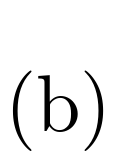
\includegraphics{figures/(b).png}

}

}

\end{minipage}%
%
\begin{minipage}[t]{0.01\linewidth}

{\centering 

~

}

\end{minipage}%
%
\begin{minipage}[t]{0.45\linewidth}

{\centering 

\raisebox{-\height}{

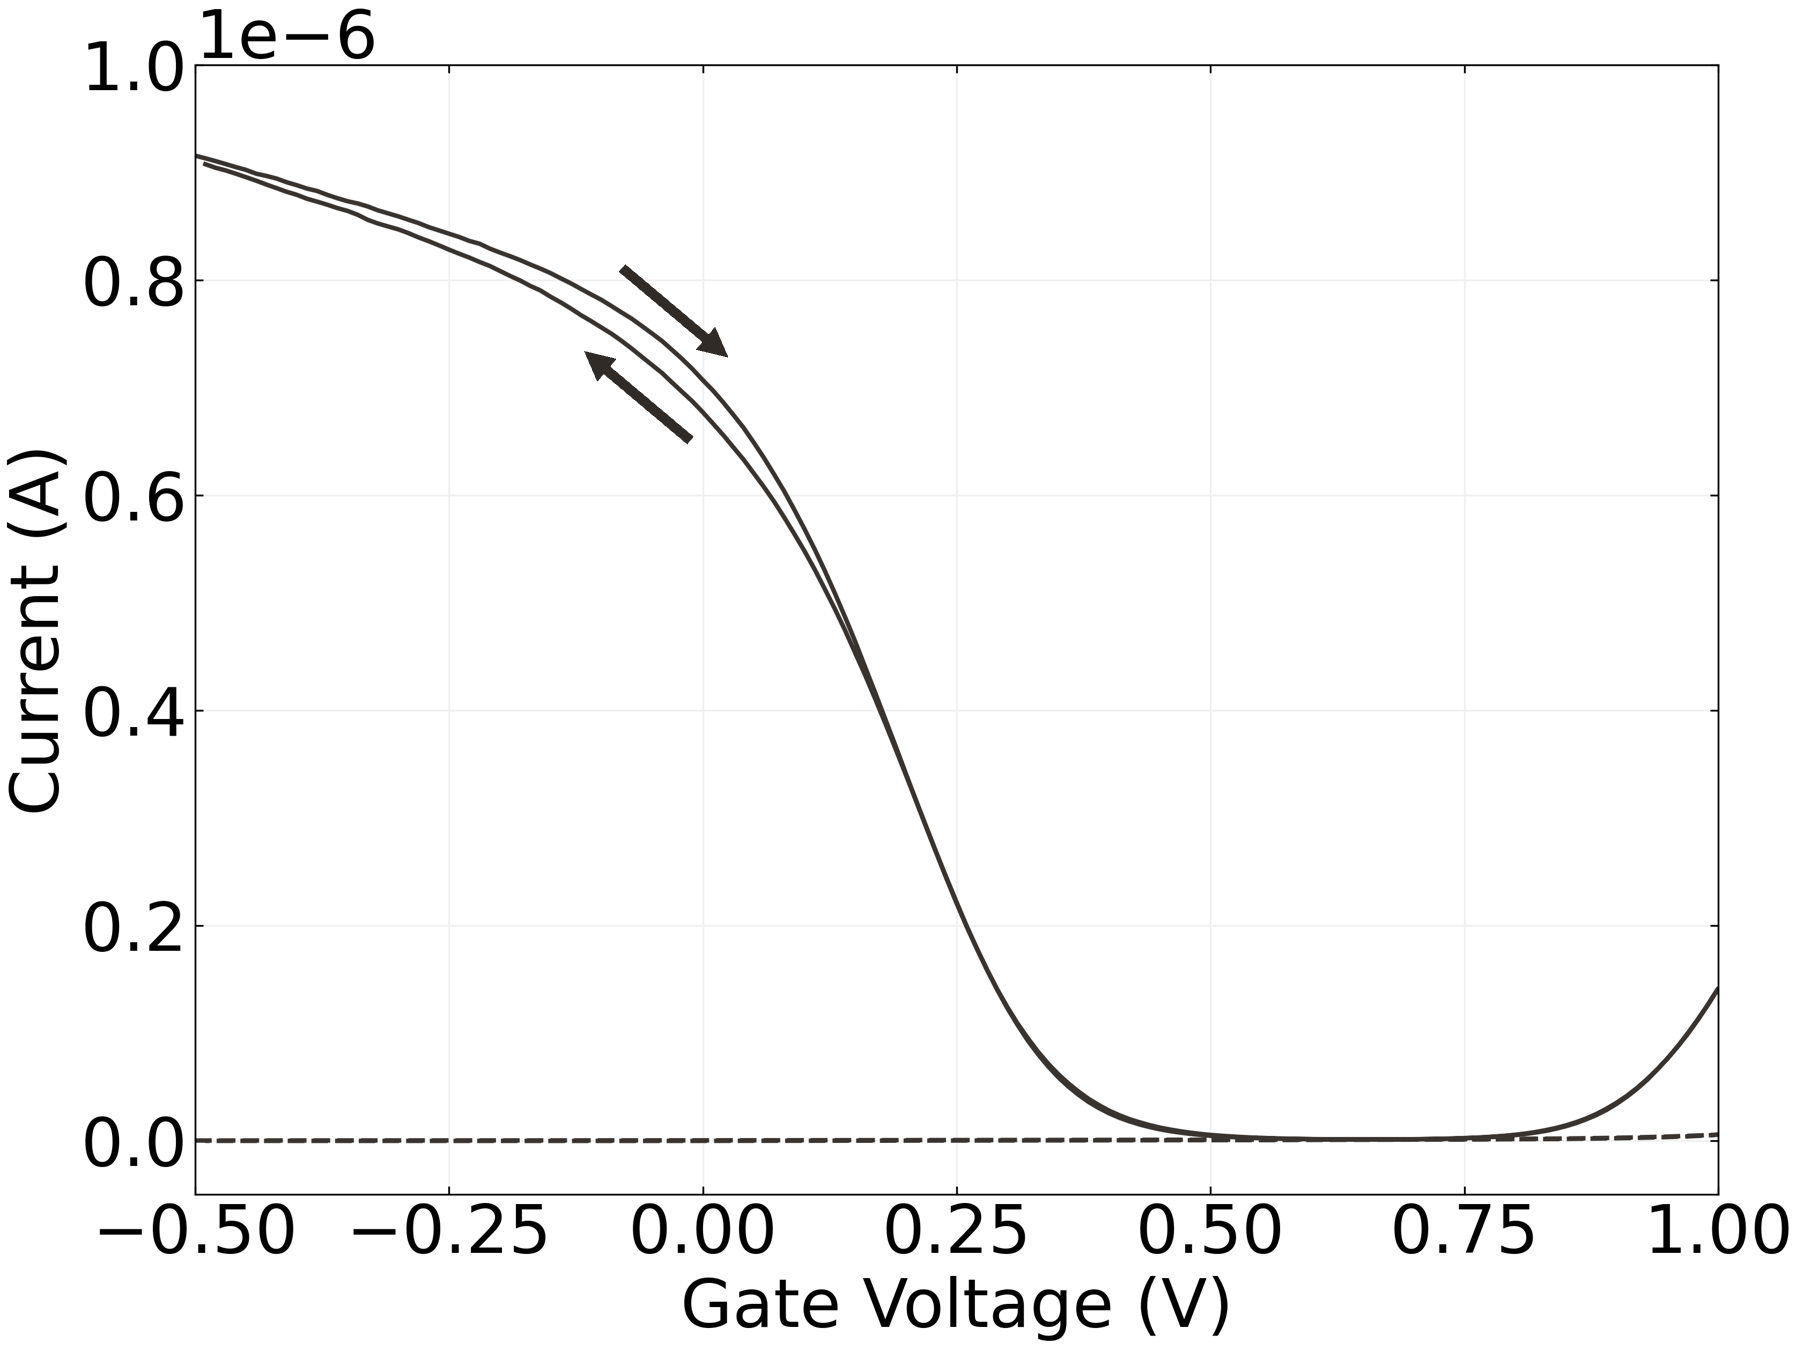
\includegraphics{figures/ch2/NTQ31C5_hysteresis.png}

}

}

\end{minipage}%
%
\begin{minipage}[t]{0.01\linewidth}

{\centering 

~

}

\end{minipage}%

\caption{\label{fig-gating-hysteresis}Field-effect transistor transfer
characteristics taken at \(V_{ds}\) = 100 mV from two different device
channels on a linear scale. Forward and reverse sweeps are shown for the
back-gated case (a) and the liquid-gated case (b), with the direction of
each sweep indicated by an arrow. A sweep rate of \(V_{ds}\) = 100
mV/sample was used for the back-gated device and a sweep rate of
\(V_{ds}\) = 10 mV/sample was used for the liquid-gate device. The gate
current measured during each sweep is also shown with a dotted line.}

\end{figure}

\hypertarget{hysteresis-and-baseline-drift}{%
\subsubsection*{Hysteresis and Baseline
Drift}\label{hysteresis-and-baseline-drift}}
\addcontentsline{toc}{subsubsection}{Hysteresis and Baseline Drift}

Thin-film transistor devices typically exhibit some degree of
hysteresis, where the history of channel current affects future current
behaviour. Hysteresis in carbon nanotube and graphene field-effect
transistors is a result of filling or emptying of slow-discharge charge
traps in the local environment of the channel. These charge traps exist
either within the silicon dioxide insulator or at its interface with the
channel, which can result from adsorption of water or other dopants
\autocite{McEuen2002,Kim2003,Wang2010}. A capacitive gating effect from
charged ions also contributes to hysteresis, either due to the use of a
electrolyte-gated environment or from charged surface contamination
\autocite{Wang2010,Yao2021}. Due to hysteresis, sweeping \(V_g\)
forwards across a set voltage range will result in a different
\(I_d - V_g\) characteristic curve than if \(V_g\) is subsequently swept
in the reverse direction over that same range. Hysteresis depends on the
voltage range used for characterisation, the sweep rate and the
environment of the transistor channel \autocite{Kim2003,Wang2010}. The
difference between the forward and reverse sweep for both the back-gated
and liquid-gated case is illustrated in
Figure~\ref{fig-gating-hysteresis}. The hysteresis is significantly
lower for the liquid-gated case, which may be explained by the reduced
voltage range and sweep rate. However, the electrolyte layer may also
prevent atmospheric adsorbents reaching the channel, further reducing
hysteresis.

Memory effects are also present during current measurement when both
source-drain and source-gate voltages are kept constant. These changes
appear as a slow change in current, and are referred to here as either
signal drift or baseline drift. In more extreme cases, baseline drift
can obscure or even be confused with current changes attributable to
analyte interaction during real-time sensing. Signal drift occurs both
in ambient conditions and in a vacuum environment, and cannot be
accounted for by changes in room temperature and ambient lighting alone.
While research into signal drift is ongoing, it appears to be a
hysteretic effect resulting from the filling of trap states over time
\autocite{Lin2006,Noyce2019}. The high demand for characterisation
equipment in a standard device laboratory means that waiting over three
hours for baseline drift to settle is impractical, and furthermore,
extended periods of voltage application may degrade bio-functionalised
devices \autocite{Noyce2019}. Since trap states are unavoidable to a
degree \autocite{DiMaria1993,Collins2000}, data analysis that accounts
for baseline drift was therefore explored in some detail in this thesis.

\hypertarget{graphene-field-effect-transistors}{%
\section{Graphene Field-Effect
Transistors}\label{graphene-field-effect-transistors}}

\hypertarget{graphene-properties}{%
\subsection{Graphene Properties}\label{graphene-properties}}

Graphene is a 2-dimensional material which consists of covalently bonded
carbon atoms in a dense lattice of hexagonal cells
\autocite{McEuen2002,Novoselov2004,Geim2007,Tran2016}. Graphene can be
used to create a variety of low-dimensional graphitic nanomaterials,
including carbon nanotubes \autocite{McEuen2002} (see
Section~\ref{sec-carbon-nanotubes}). Monolayer and bilayer graphene are
zero band-gap semiconductors, where traversing the electronic
bandstructure in different directions gives rise to either metallic or
semiconducting behaviour \autocite{McEuen2002}. Adding more graphene
layers adds more complexity to the bandstructure, with significant
overlap between bands and reduced carrier mobility. When 10 or more
layers are present, the structure behaves as 3D graphite
\autocite{Geim2007,Ohno2015}. First isolated in 2004
\autocite{Novoselov2004}, monolayer graphene has many desirable
electronic properties. Charge carrier transport is ballistic over
submicrometer distances at room temperature, and as graphene is metallic
even at the Dirac point, this transport is not inhibited by a Schottky
barrier at the metal contacts of a device
\autocite{Novoselov2004,Geim2007}. Graphene is also a highly chemically
stable material. In particular, it will not readily oxidise in an
electrolyte solution due to having a large `electrochemical window'; in
other words, it is too chemically stable to take part in electrochemical
reactions within a large range of applied voltages
\autocite{Ohno2015,Tran2016}.

\hypertarget{graphene-folds}{%
\subsubsection*{Graphene Folds}\label{graphene-folds}}
\addcontentsline{toc}{subsubsection}{Graphene Folds}

Vertical warping on the scale of tens of nanometers helps to stablise
the graphene layer, increasing elastic energy but reducing the thermal
vibrations which are large in a 2D material \autocite{Geim2007}.

\hypertarget{sec-electrical-characterisation-graphene}{%
\subsection{Electrical
Characterisation}\label{sec-electrical-characterisation-graphene}}

\begin{figure}

\begin{minipage}[t]{0.03\linewidth}

{\centering 

\raisebox{-\height}{

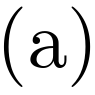
\includegraphics{figures/(a).png}

}

}

\end{minipage}%
%
\begin{minipage}[t]{0.01\linewidth}

{\centering 

~

}

\end{minipage}%
%
\begin{minipage}[t]{0.45\linewidth}

{\centering 

\raisebox{-\height}{

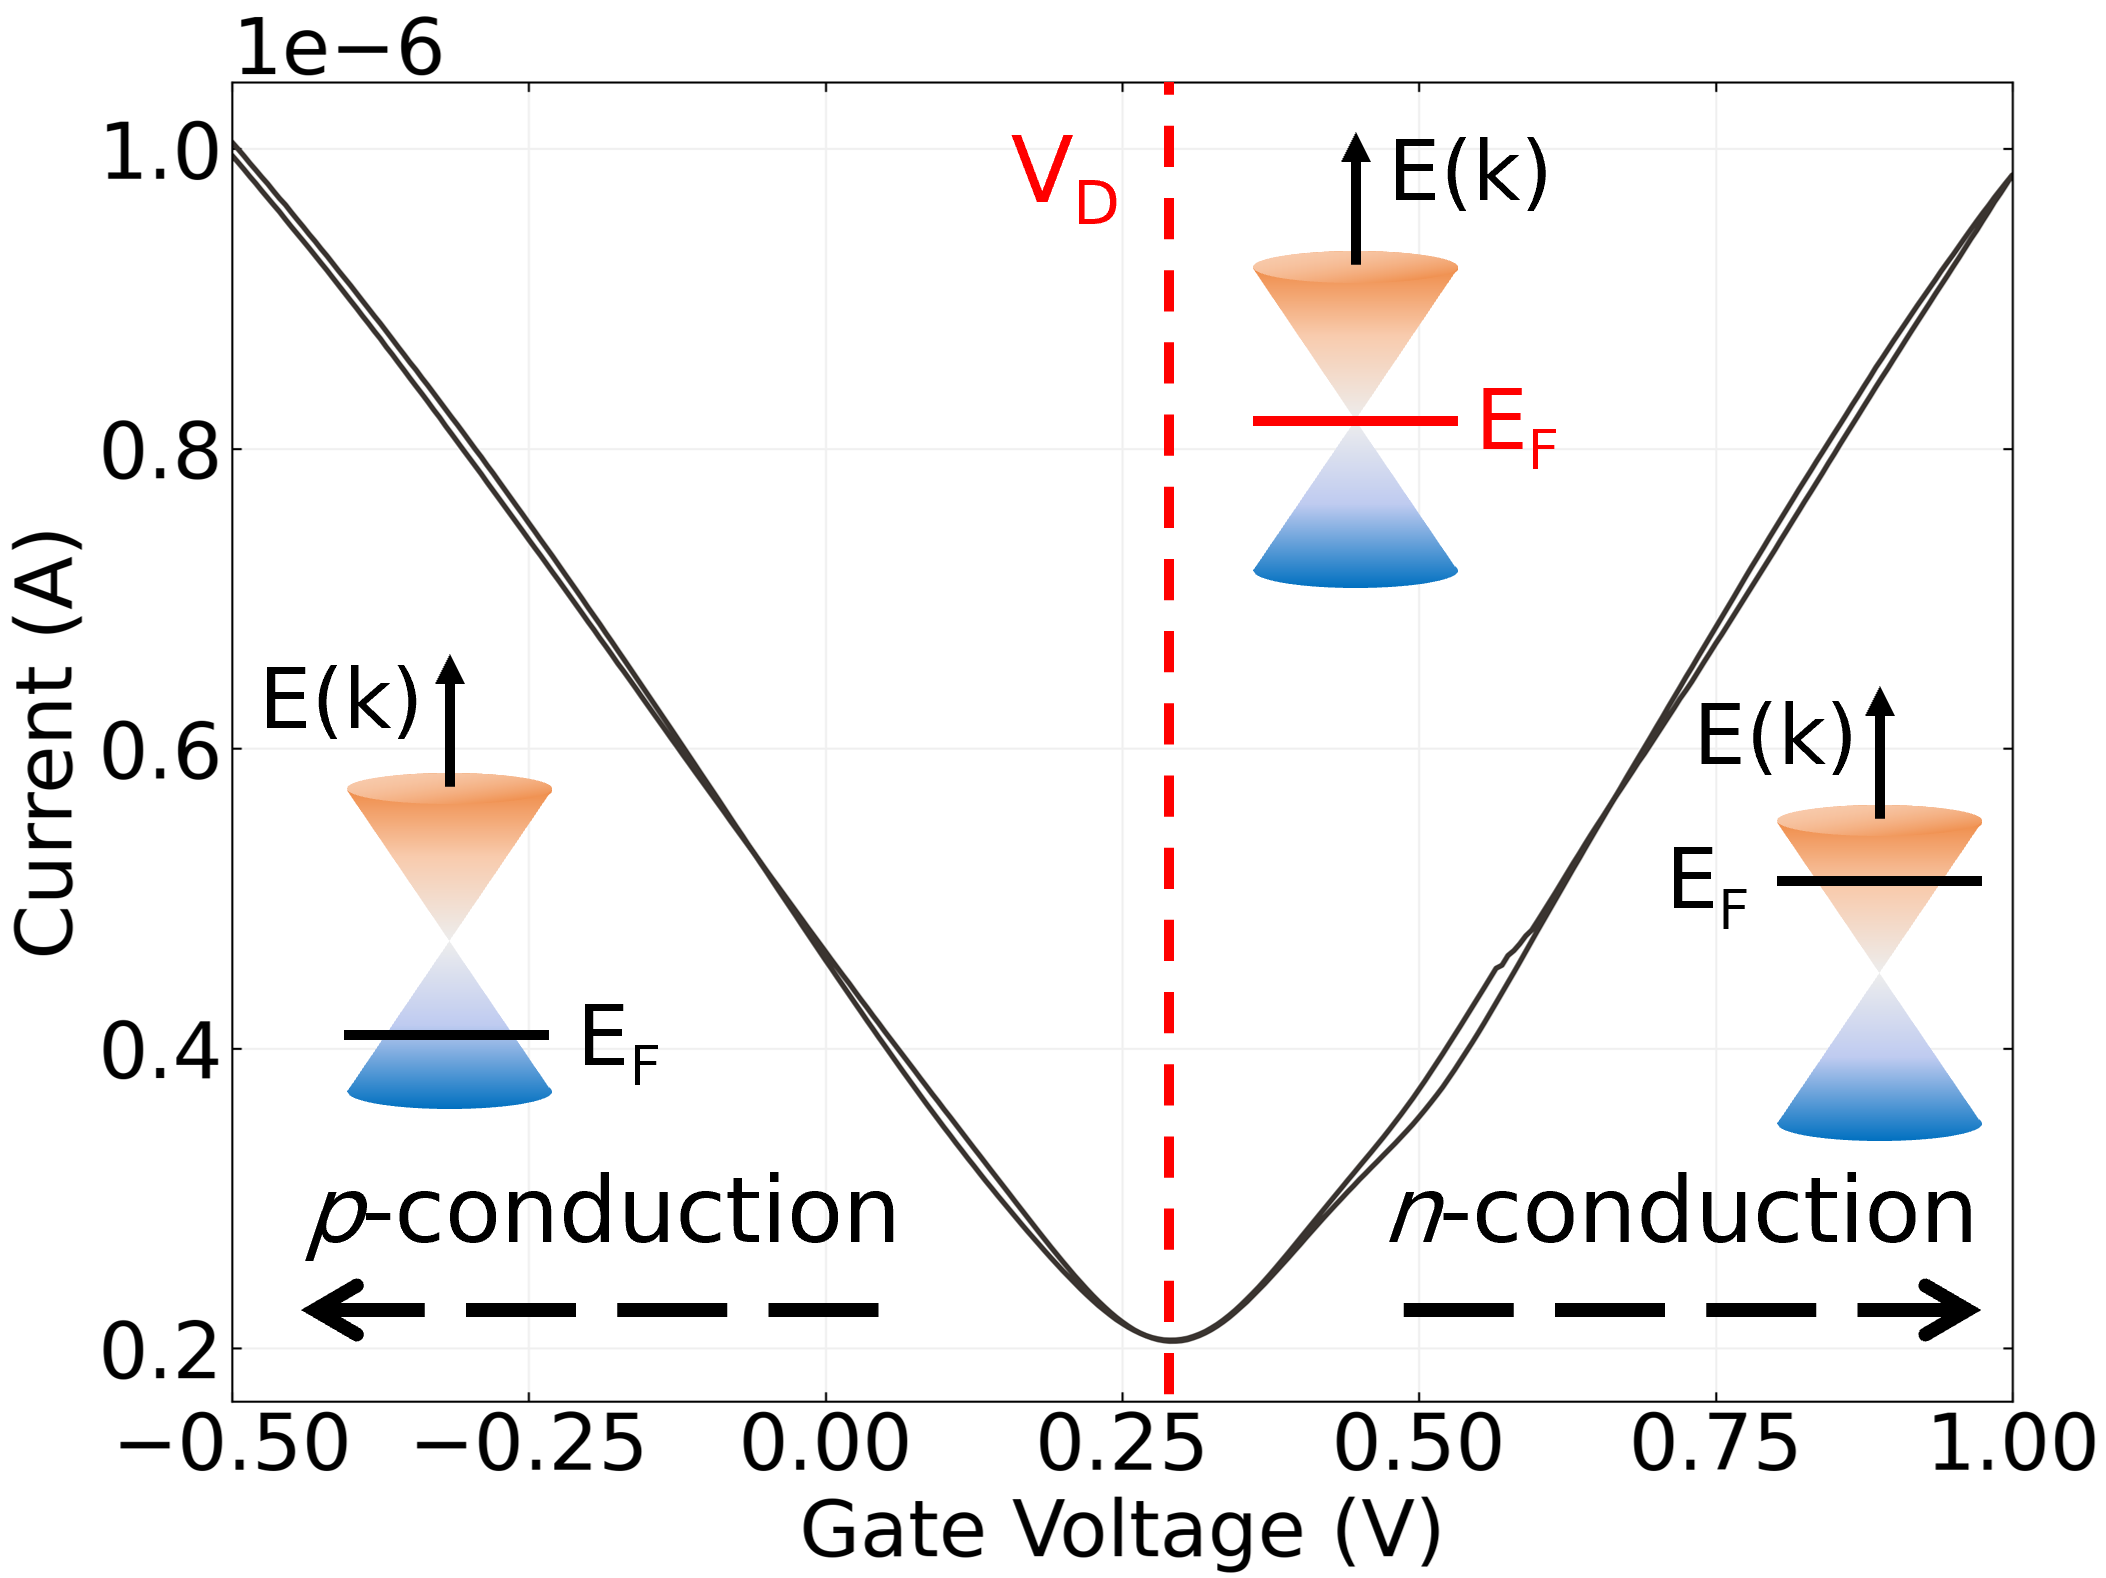
\includegraphics{figures/ch2/Graphene_transfer_1.png}

}

}

\end{minipage}%
%
\begin{minipage}[t]{0.01\linewidth}

{\centering 

~

}

\end{minipage}%
%
\begin{minipage}[t]{0.03\linewidth}

{\centering 

\raisebox{-\height}{

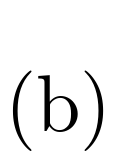
\includegraphics{figures/(b).png}

}

}

\end{minipage}%
%
\begin{minipage}[t]{0.01\linewidth}

{\centering 

~

}

\end{minipage}%
%
\begin{minipage}[t]{0.45\linewidth}

{\centering 

\raisebox{-\height}{

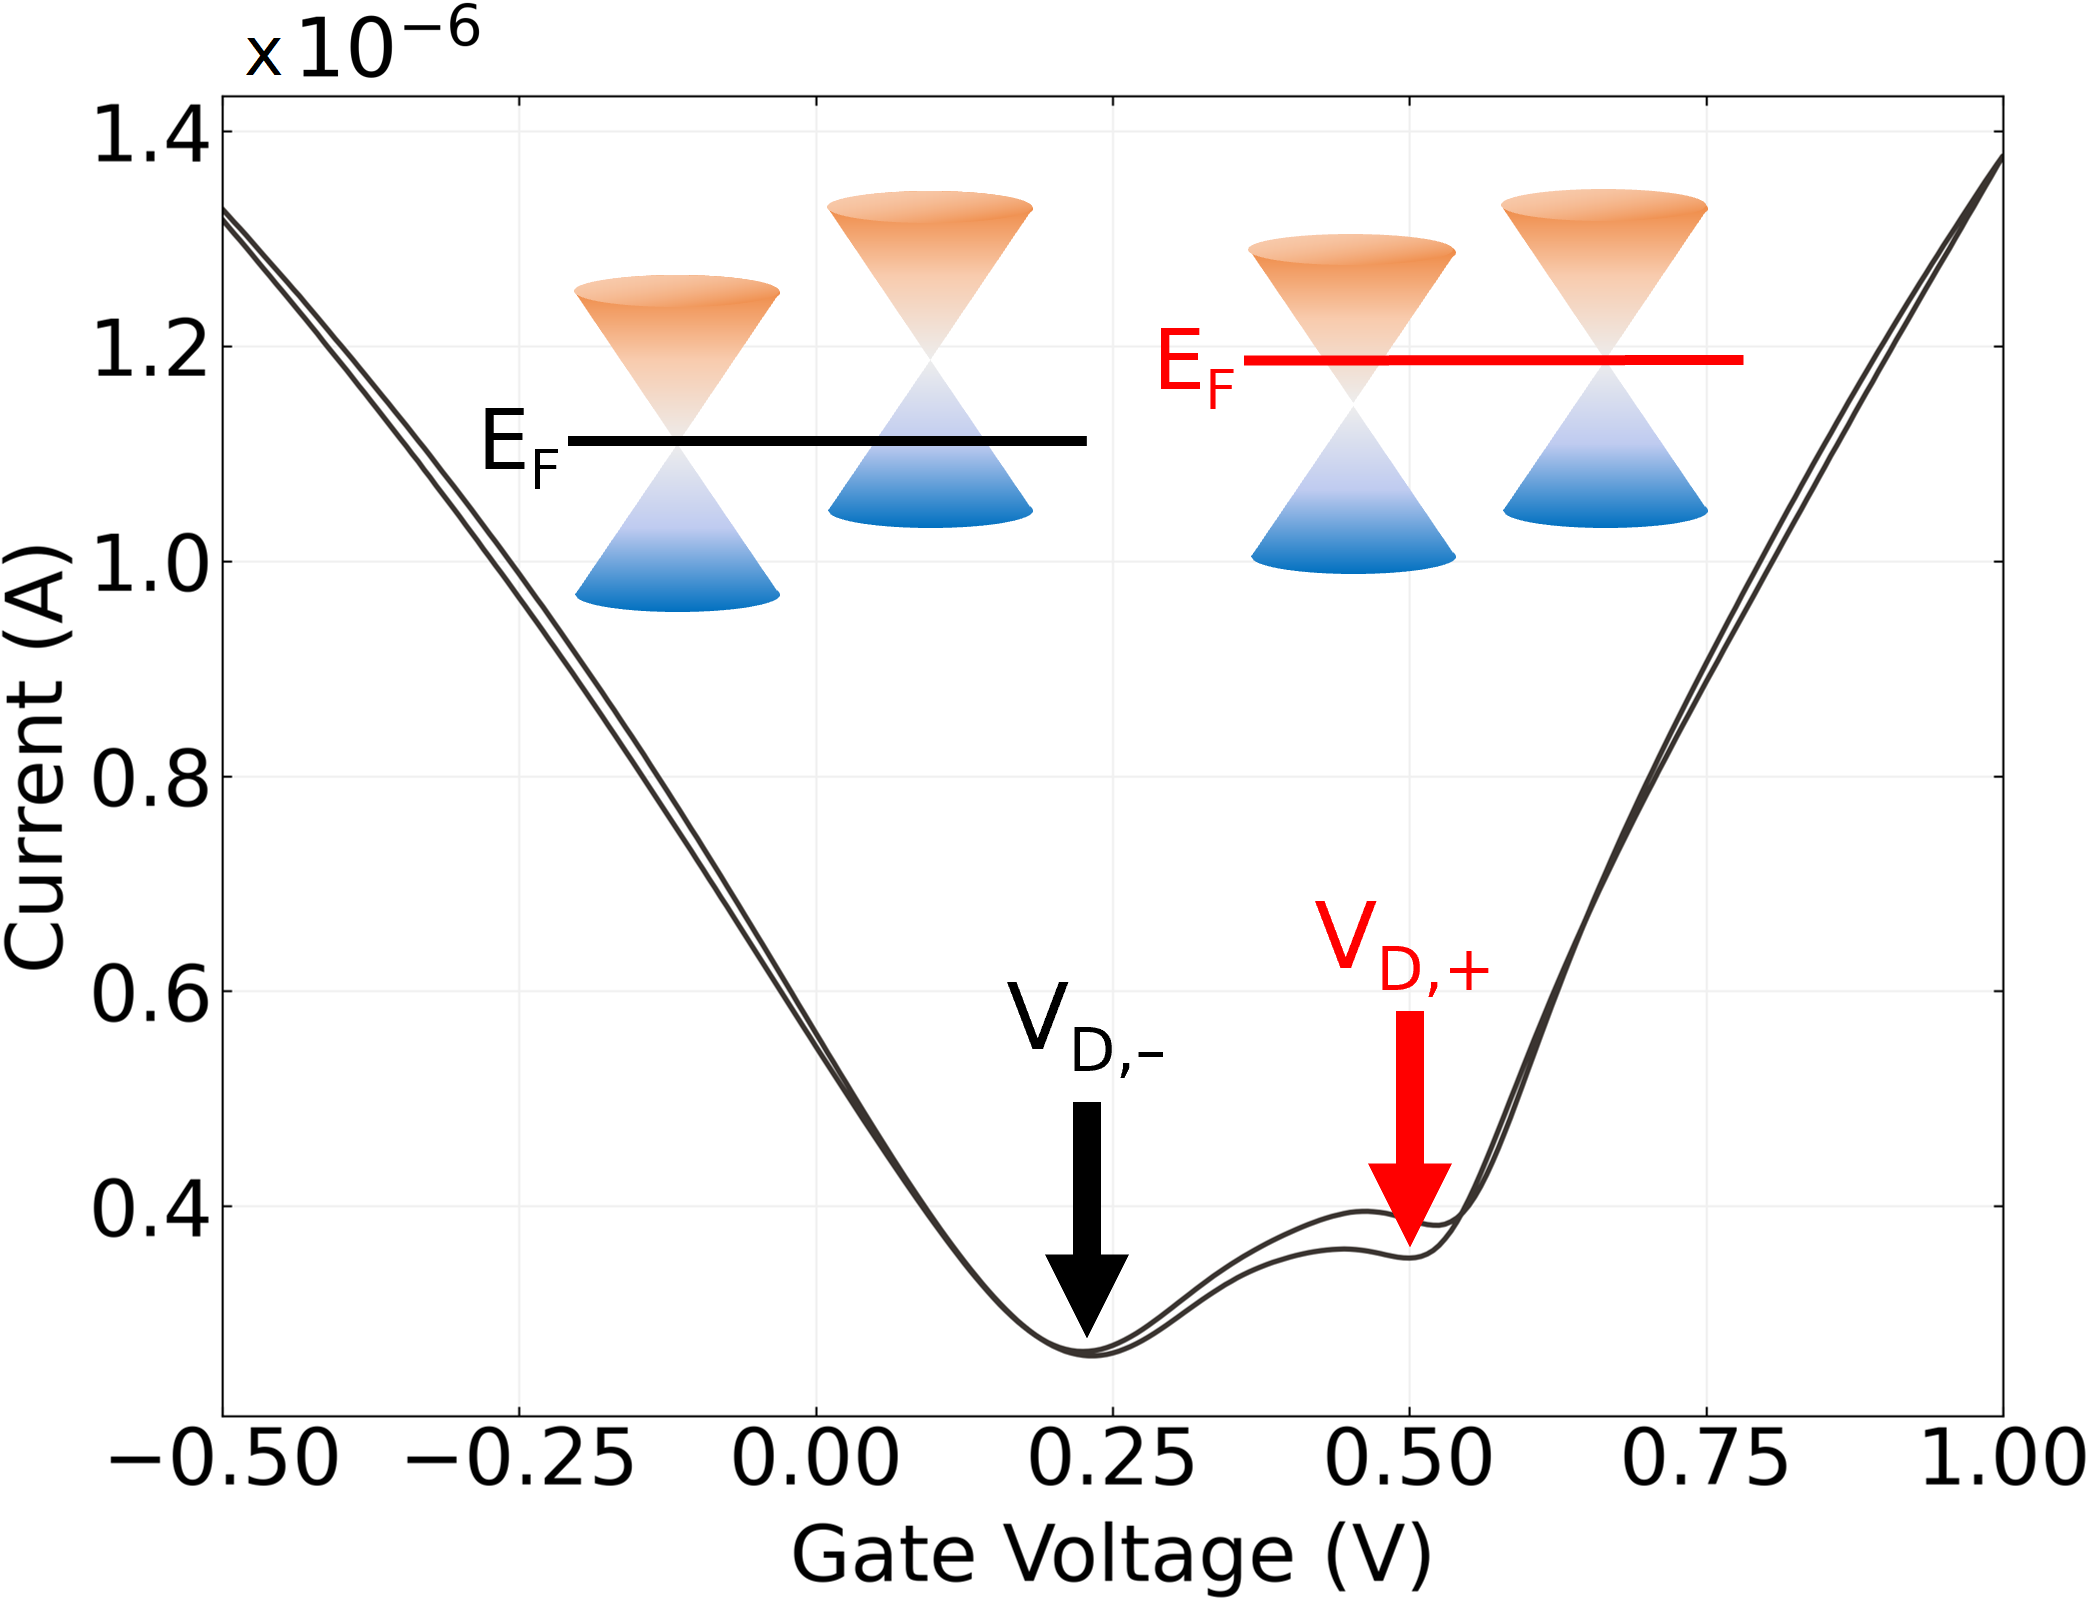
\includegraphics{figures/ch2/Graphene_transfer_2.png}

}

}

\end{minipage}%
%
\begin{minipage}[t]{0.01\linewidth}

{\centering 

~

}

\end{minipage}%

\caption{\label{fig-graphene-characteristics}Liquid-gated transfer
characteristics of two graphene field-effect transistor channels. In
(a), the Dirac point voltage is indicated by a red dotted line, and
regions of hole conduction and electron conduction are also shown. The
relative Fermi energy in each region is shown on graphene bandstructure
insets (adapted from \autocite{Geim2007,Ohno2015}). The graphene channel
in (b) has double conduction minima, which are highlighted with red
arrows.}

\end{figure}

When a gate voltage \(V_g\) is applied to the channel of a graphene
device, the Fermi energy of the graphene is shifted and surface charge
density is altered \autocite{Novoselov2004,Heller2010,Ohno2015}. An
increase in available charge means an increase in carriers available for
conduction and increased \(I_d\) \autocite{Geim2007}.

The transfer sweep behaviour is that of an ambipolar semiconductor,
except there is no characteristic `off' regime. The minimum conductance
obtainable by gating occurs at what is known as the neutrality or Dirac
point, where the population of charge carriers is at a minimum
\autocite{Novoselov2004,Ohno2015}. At voltages close to the Dirac
voltage, a mixed state exists where both electrons and holes are
present. As gate voltage moves left away from the Dirac voltage, holes
begin to dominate conduction, while when gate voltage is moved to the
right of the Dirac voltage, electrons dominate \autocite{Novoselov2004}.

As gate voltage is increased or decreased away from the Dirac voltage,
conductivity increases linearly \autocite{Novoselov2004}. Typically, a
monolayer graphene channel will conduct holes at zero gate voltage,
which is due to the presence of atmospheric dopants such as water. By
removing these dopants, the Dirac point feature can be brought closer to
the zero gate voltage position on the transfer curve, indicating
graphene is naturally a mixed-carrier conductor
\autocite{Novoselov2004}.

The on-off ratio of the graphene transfer curve shown is 5. As graphene
lacks a bandgap, there is a minimum possible conductance for graphene
devices, which leads to a relatively small on-off ratio
\autocite{Novoselov2004,Geim2007}. This attribute is a drawback of the
graphene FET in sensing applications when compared with carbon nanotube
transistors \autocite{Novoselov2004}. However, the transconductance of
the curve at \(V_g\) = 0 V, \(g_m\) = 1 µS, is similar to the
liquid-gated transconductance of a carbon nanotube device shown earlier.

while the Dirac voltage is 0.29 V.

Quantative measurement of leftward shift in transfer curve

I compared the transfer characteristics after then rinse steps to the
pristine characteristics Transfer shifts where current drops to zero are
excluded (indicates delamination/damage to channel)

\hypertarget{sensing-mechanisms}{%
\subsection{Sensing Mechanisms}\label{sensing-mechanisms}}

The large surface-to-volume ratio of graphene makes it highly sensitive
to intermolecular interactions and therefore appropriate for use in
sensing applications \autocite{Ohno2015,Tran2016}. An analyte molecule
can be detected using a graphene channel by observing the change in
current that occurs when a charged analyte alters the channel Fermi
level \autocite{Heller2010,Ohno2015}.

\hypertarget{random-network-carbon-nanotube-field-effect-transistors}{%
\section{Random-Network Carbon Nanotube Field-Effect
Transistors}\label{random-network-carbon-nanotube-field-effect-transistors}}

\hypertarget{sec-carbon-nanotubes}{%
\subsection{Carbon Nanotube Properties}\label{sec-carbon-nanotubes}}

Since their initial identification in 1991 \autocite{Iijima1991}, a wide
range of applications for carbon nanotubes (CNTs) have been proposed,
due to their small mass, elasticity, strength, and unique electronic
properties. A single-walled carbon nanotube (SWCNT) consists of a
monolayer graphene sheet rolled up into a cylinder, while a multi-walled
carbon nanotube (MWCNT) consists of several monolayer graphene cylinders
where smaller cylinders are coaxially contained by larger cylinders
\autocite{Dekker1999,Avouris2007,Cao2009,Rouhi2010,Shkodra2021}.
Multi-walled carbon nanotubes can suffer from significant scattering at
defects leading to diffusive electron motion \autocite{Dekker1999}.
However, single-walled carbon nanotubes are relatively defect-free, and
carrier transport within nanotubes is near-ballistic at room
temperature, resulting in high carrier mobility
\autocite{Dekker1999,Avouris2007,Cao2009,Rouhi2010,Shkodra2021}. The
momentum of charge carriers in a single-walled carbon nanotube is
quantised, confining carriers to 2-dimensional slices across the
3-dimensional graphene bandstructure. If a slice contains a bandgap, the
carbon nanotube behaves as a semiconductor (s-CNT); if not, the nanotube
behaves as a metal (m-CNT) \autocite{McEuen2002}. The high
surface-to-volume ratio of small-diameter single-walled carbon nanotubes
makes them extremely sensitive and therefore particularly suitable for
sensing applications \autocite{Cao2009,Yao2021,Shkodra2021}. Like
graphene, carbon nanotubes have a large potential window, and can be
used safely in a liquid-gate environment without undergoing redox
reactions \autocite{Ohno2015}.

\begin{figure}

{\centering 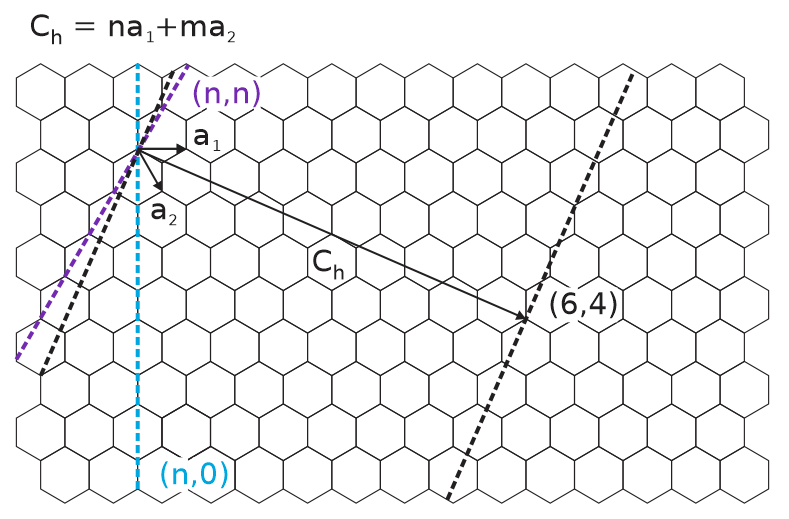
\includegraphics[width=0.7\textwidth,height=\textheight]{figures/ch2/carbon_nanotube_wrapping.png}

}

\caption{\label{fig-carbon-nanotube-wrapping}Diagram illustrating how a
graphene sheet can be rolled up at various angles to form carbon
nanotubes. The two black dotted lines represent boundaries which can be
cut across and then brought into contact to form a cylinder. The
cylinder here is referred to by the integer pair (6,4), as the chiral
vector \(C_h\), the vector perpendicular to the cut through the sheet,
is given by \(C_h = 6a_1+4a_2\). The chiral vector forms the
circumference of the rolled carbon nanotube. The left edge in the zigzag
(\(n\),0) and armchair (\(n\),\(n\)) cases are shown with a blue and
purple dotted line respectively. The location of the right edge
(diameter of the nanotube) is determined by the value chosen for \(n\).
Adapted from \autocite{Dekker1999,Lu2012}.}

\end{figure}

The chirality and diameter of a carbon nanotube determines its
electronic bandstructure and whether it has semiconducting or metallic
characteristics
\autocite{Martel1998,Dekker1999,McEuen2002,Avouris2007,Shkodra2021,Li2023}.
The chirality indices of a nanotube (\(n\),\(m\)) determines the chiral
angle at which hexagons wind around the nanotube relative to the
longitudinal axis of the nanotube. This chiral angle is the angle
between the chiral vector
\(\textbf{C}_h = n\textbf{a}_1+m\textbf{a}_2\), which maps to the
circumference of the nanotube, and the basis vector \(\textbf{a}_1\),
which is parallel to a row of hexagons. The size of the chiral angle
\(\theta\) is given by Equation~\ref{eq-chiral-angle}, the diameter of
the resulting carbon nanotube is given by \(d=|C_h|/\pi\)
\autocite{Lu2012}.

\begin{equation}\protect\hypertarget{eq-chiral-angle}{}{
\theta = \arcsin\frac{\sqrt{3}m}{2\sqrt{n^2+nm+m^2}}, \space n > m
}\label{eq-chiral-angle}\end{equation}

When \(m=0\), \(\theta = 0°\), and the resulting carbon nanotube has a
`zigzag' structure; when \(m=n\), \(\theta = 30°\), and the carbon
nanotube has an `armchair' structure. When \(\theta\) is between
\(0°-30°\), the structure is referred to as `chiral'
\autocite{Dekker1999,Lu2012}. When \(n-m=3z\), where \(z\) is an
integer, the resulting carbon nanotube is metallic \(-\) for example, if
\(n=5\) and \(m=5\), \(z=0\), therefore the tube is metallic. All other
nanotubes are semiconducting, including the (6,4) chiral nanotube
described in Figure~\ref{fig-carbon-nanotube-wrapping}. Out of the
chiral arrangements available, two-thirds of the possible structures are
semiconducting while one-third is metallic \autocite{Dekker1999}.

\hypertarget{carbon-nanotube-networks}{%
\subsection{Carbon Nanotube Networks}\label{carbon-nanotube-networks}}

Although a single carbon nanotube can be used as the channel of a
thin-film transistor, this approach has significant drawbacks. An
alternative approach is to use a large-scale network of carbon nanotubes
as the transistor channel. Here, the individual electrical properties of
the CNTs are averaged out across the network, which minimises
device-to-device variation. Furthermore, the large area of coverage both
ensures high currents and increases the likelihood of interactions with
the local environment in sensing applications
\autocite{Hu2004,Cao2009,Murugathas2019a,Li2023}. Carbon nanotube
networks can either be aligned or randomly deposited
\autocite{Cao2009,Shkodra2021}; in this thesis, randomly deposited
networks were fabricated using facile solution-deposition methods.
Important attributes of a carbon nanotube film include the density of
the network (number of nanotubes per unit area), the ratio of metallic
to semiconducting nanotubes present, and the distribution of nanotube
diameters present \autocite{Cao2009,Shkodra2021}. The strong van der
Waals forces between carbon nanotubes lead to them bundling together
within a network. These bundles may contain many nanotubes of different
size and chirality \autocite{Fuhrer2000,Hu2004,Cao2009,Murugathas2019a}.

In a network carbon nanotube device with metal electrodes, transistor
switching is primarily governed by band bending at the interfaces
between each electrode and the semiconducting carbon nanotubes. The
difference in Fermi level between each material leads to a a flow of
charge across each interface until the Fermi levels equilibriate and a
Schottky barrier forms. These barriers are effectively electric dipole
layers, whose net electric fields restrict the further flow of charge at
each interface. This band bending process depends on the work function
of the metal, so the type of metal determines the type of charge being
restricted. For example, a high work function metal bends the valence
band of the semiconductor towards the Fermi level of the metal, creating
a low barrier for holes but a high barrier for electrons at each
interface \autocite{Avouris2007,Bargaoui2018}. For current to flow,
quantum tunnelling must occur through the Schottky barriers. If the
barrier size is low for electrons and holes, they both flow through the
channel, which is referred to as `ambipolar' behaviour. However, the
metal electrodes may cause the Schottky barriers to favour one type over
another, leading to `unipolar' conduction
\autocite{Avouris2007,Heller2008}.

The behaviour of carbon nanotube network transistors is also influenced
by a variety of potential barriers existing at junctions between carbon
nanotubes. A prominent example is the Schottky barriers existing at
junctions between metallic and semiconducting nanotubes (m-s junctions)
\autocite{Fuhrer2000,Topinka2009,Murugathas2019a}. These potential
barriers cause significantly heightened resistance at these junctions
relative to other points in the network \autocite{Fuhrer2000,Jang2015}.
When the channel length is much larger than that of individual
nanotubes, channel current must pass through junctions along percolation
pathways. If only one percolation pathway exists across a sparse
network, the network density is at the `percolation threshold'. If a
network is below the percolation threshold, the channel will not conduct
\autocite{Hu2004,Topinka2009,Jang2015}. For a fixed network density well
above percolation, if a network contains a low proportion of
semiconducting tubes, percolating pathways only containing metallic
nanotubes exist. A device with this film will be highly conductive but
cannot be gated \autocite{Fuhrer2000,Topinka2009}. Increasing the
proportion of s-CNTs present means m-s junctions become more prevalent.
The introduced Schottky barriers cause a dramatic conductance drop, and
gating becomes possible. As the proportion of s-CNTs approaches 100\%,
semiconducting pathways with no metallic junctions emerge, and
conductance sharply increases once more \autocite{Topinka2009}.

\hypertarget{sec-electrical-characterisation-CNT}{%
\subsection{Electrical
Characterisation}\label{sec-electrical-characterisation-CNT}}

\begin{figure}

\begin{minipage}[t]{0.03\linewidth}

{\centering 

\raisebox{-\height}{

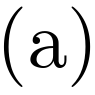
\includegraphics{figures/(a).png}

}

}

\end{minipage}%
%
\begin{minipage}[t]{0.01\linewidth}

{\centering 

~

}

\end{minipage}%
%
\begin{minipage}[t]{0.45\linewidth}

{\centering 

\raisebox{-\height}{

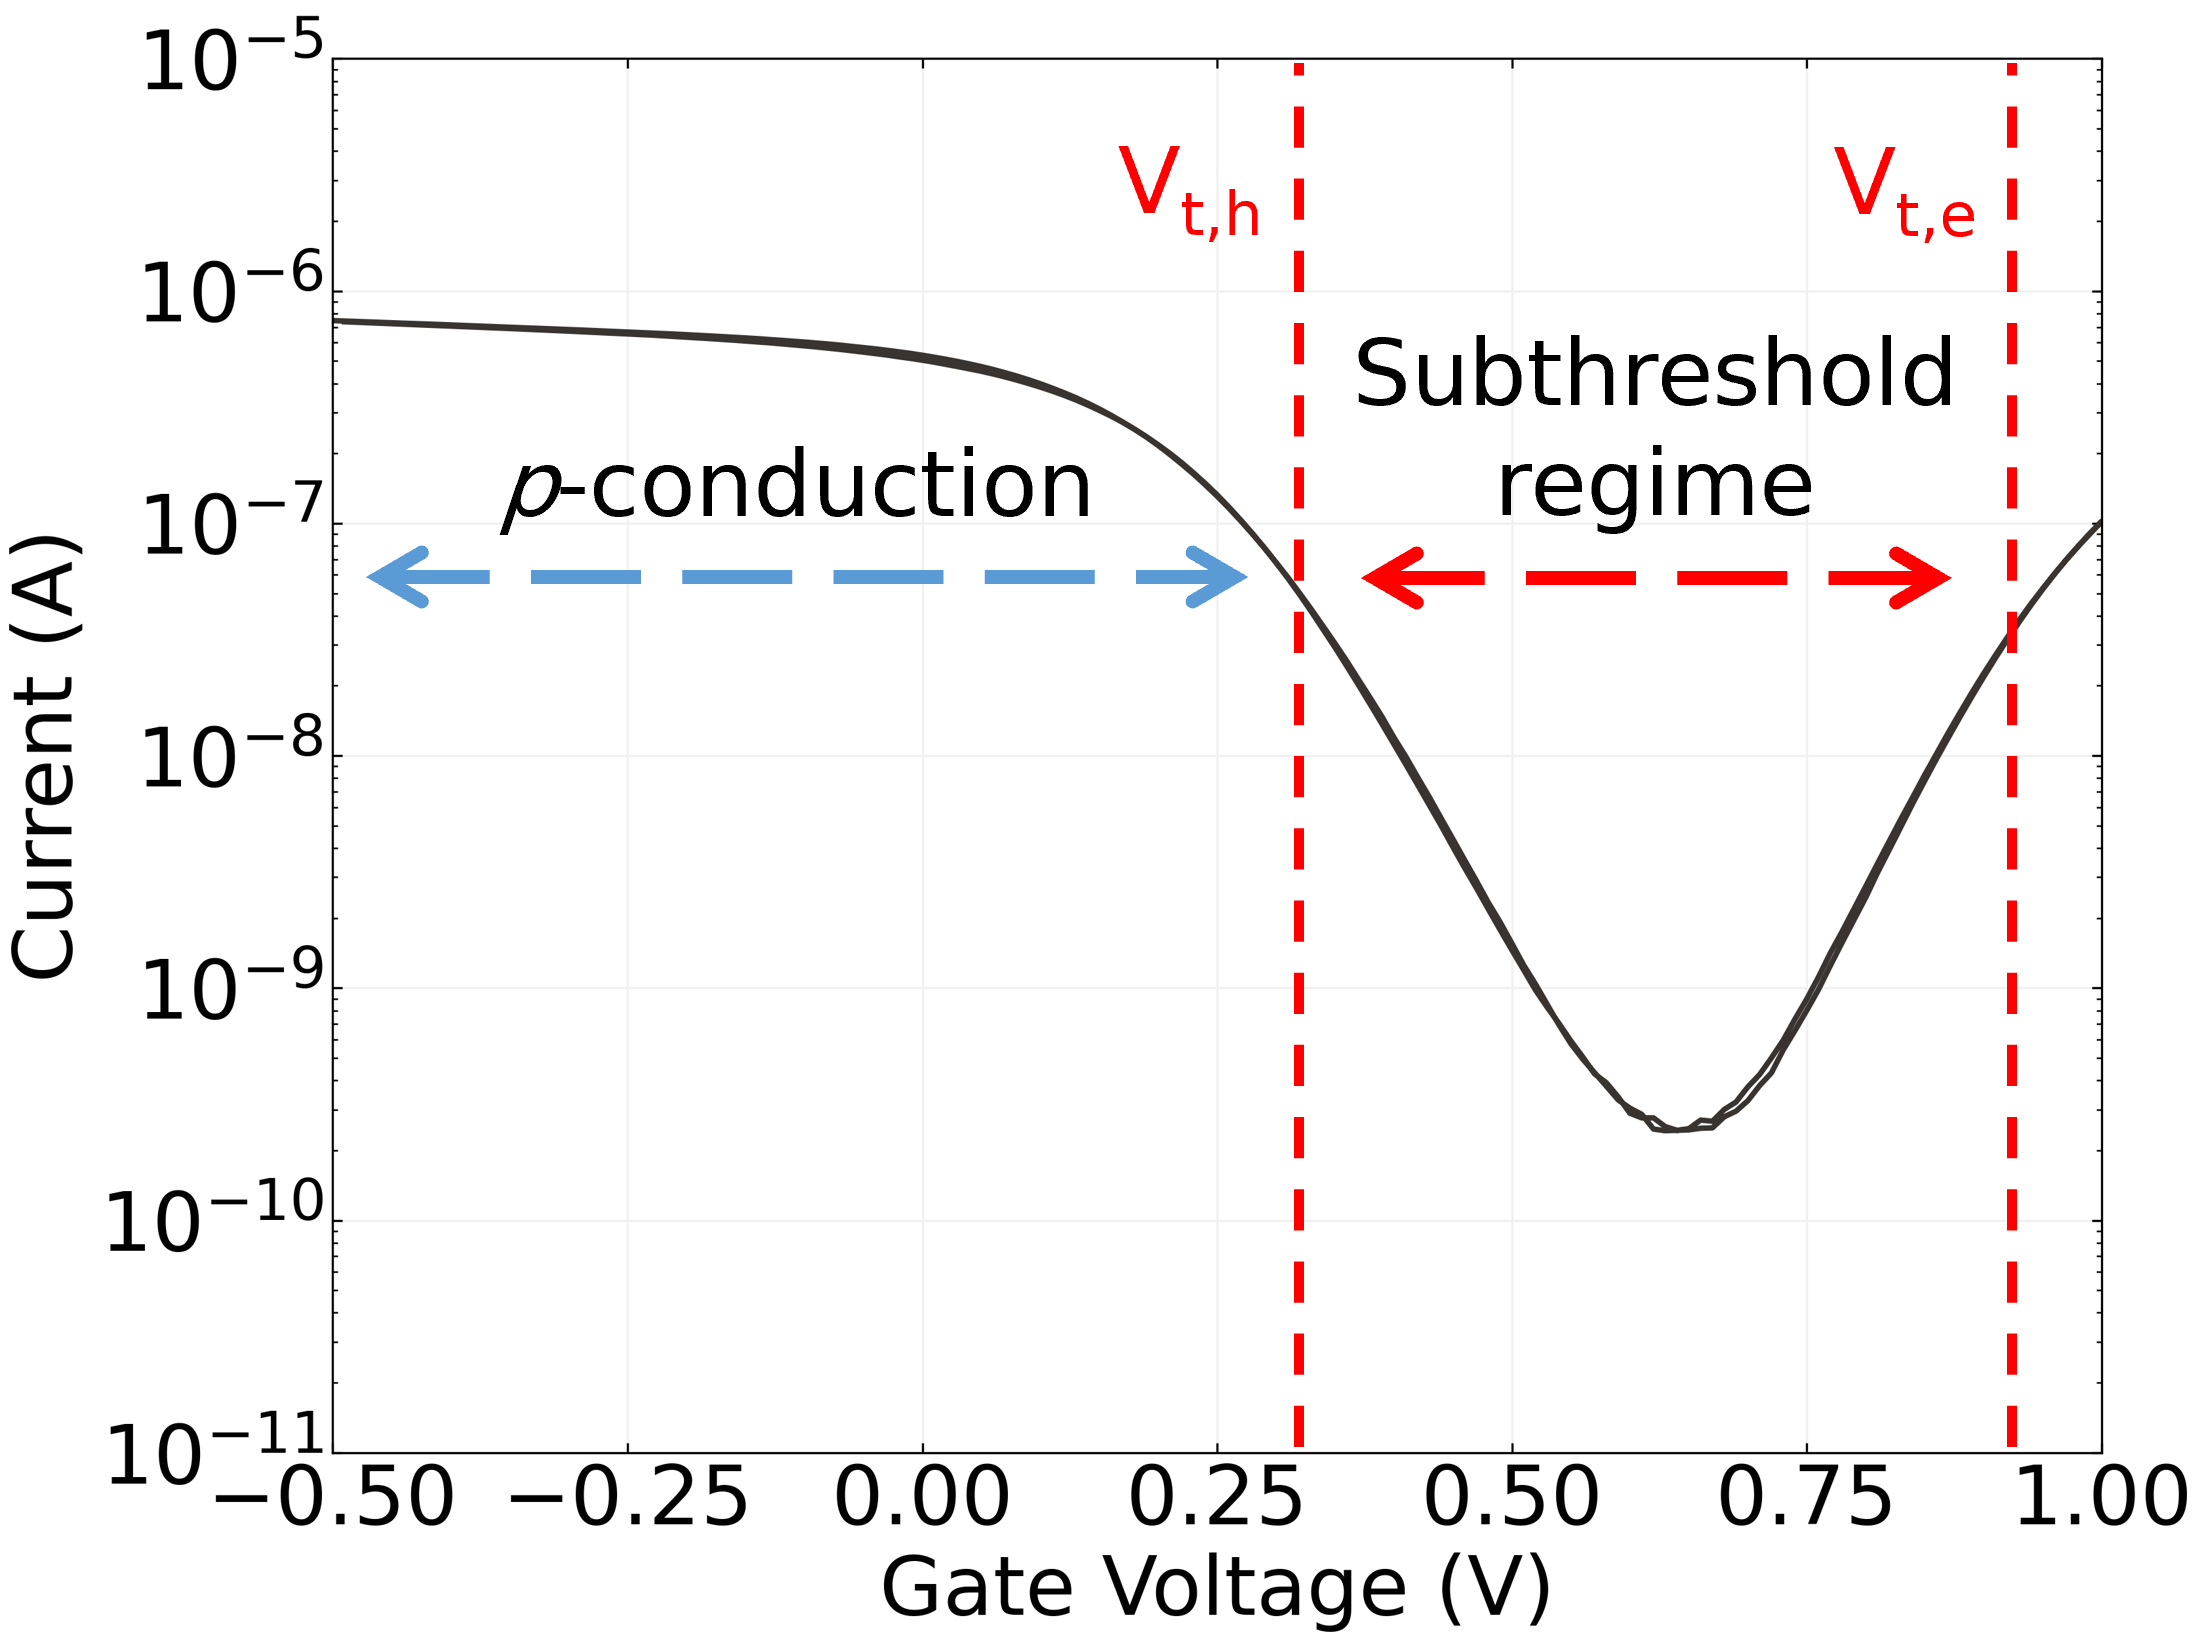
\includegraphics{figures/ch2/CNT_transfer_1.png}

}

}

\end{minipage}%
%
\begin{minipage}[t]{0.01\linewidth}

{\centering 

~

}

\end{minipage}%
%
\begin{minipage}[t]{0.03\linewidth}

{\centering 

\raisebox{-\height}{

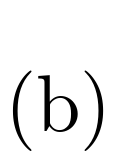
\includegraphics{figures/(b).png}

}

}

\end{minipage}%
%
\begin{minipage}[t]{0.01\linewidth}

{\centering 

~

}

\end{minipage}%
%
\begin{minipage}[t]{0.45\linewidth}

{\centering 

\raisebox{-\height}{

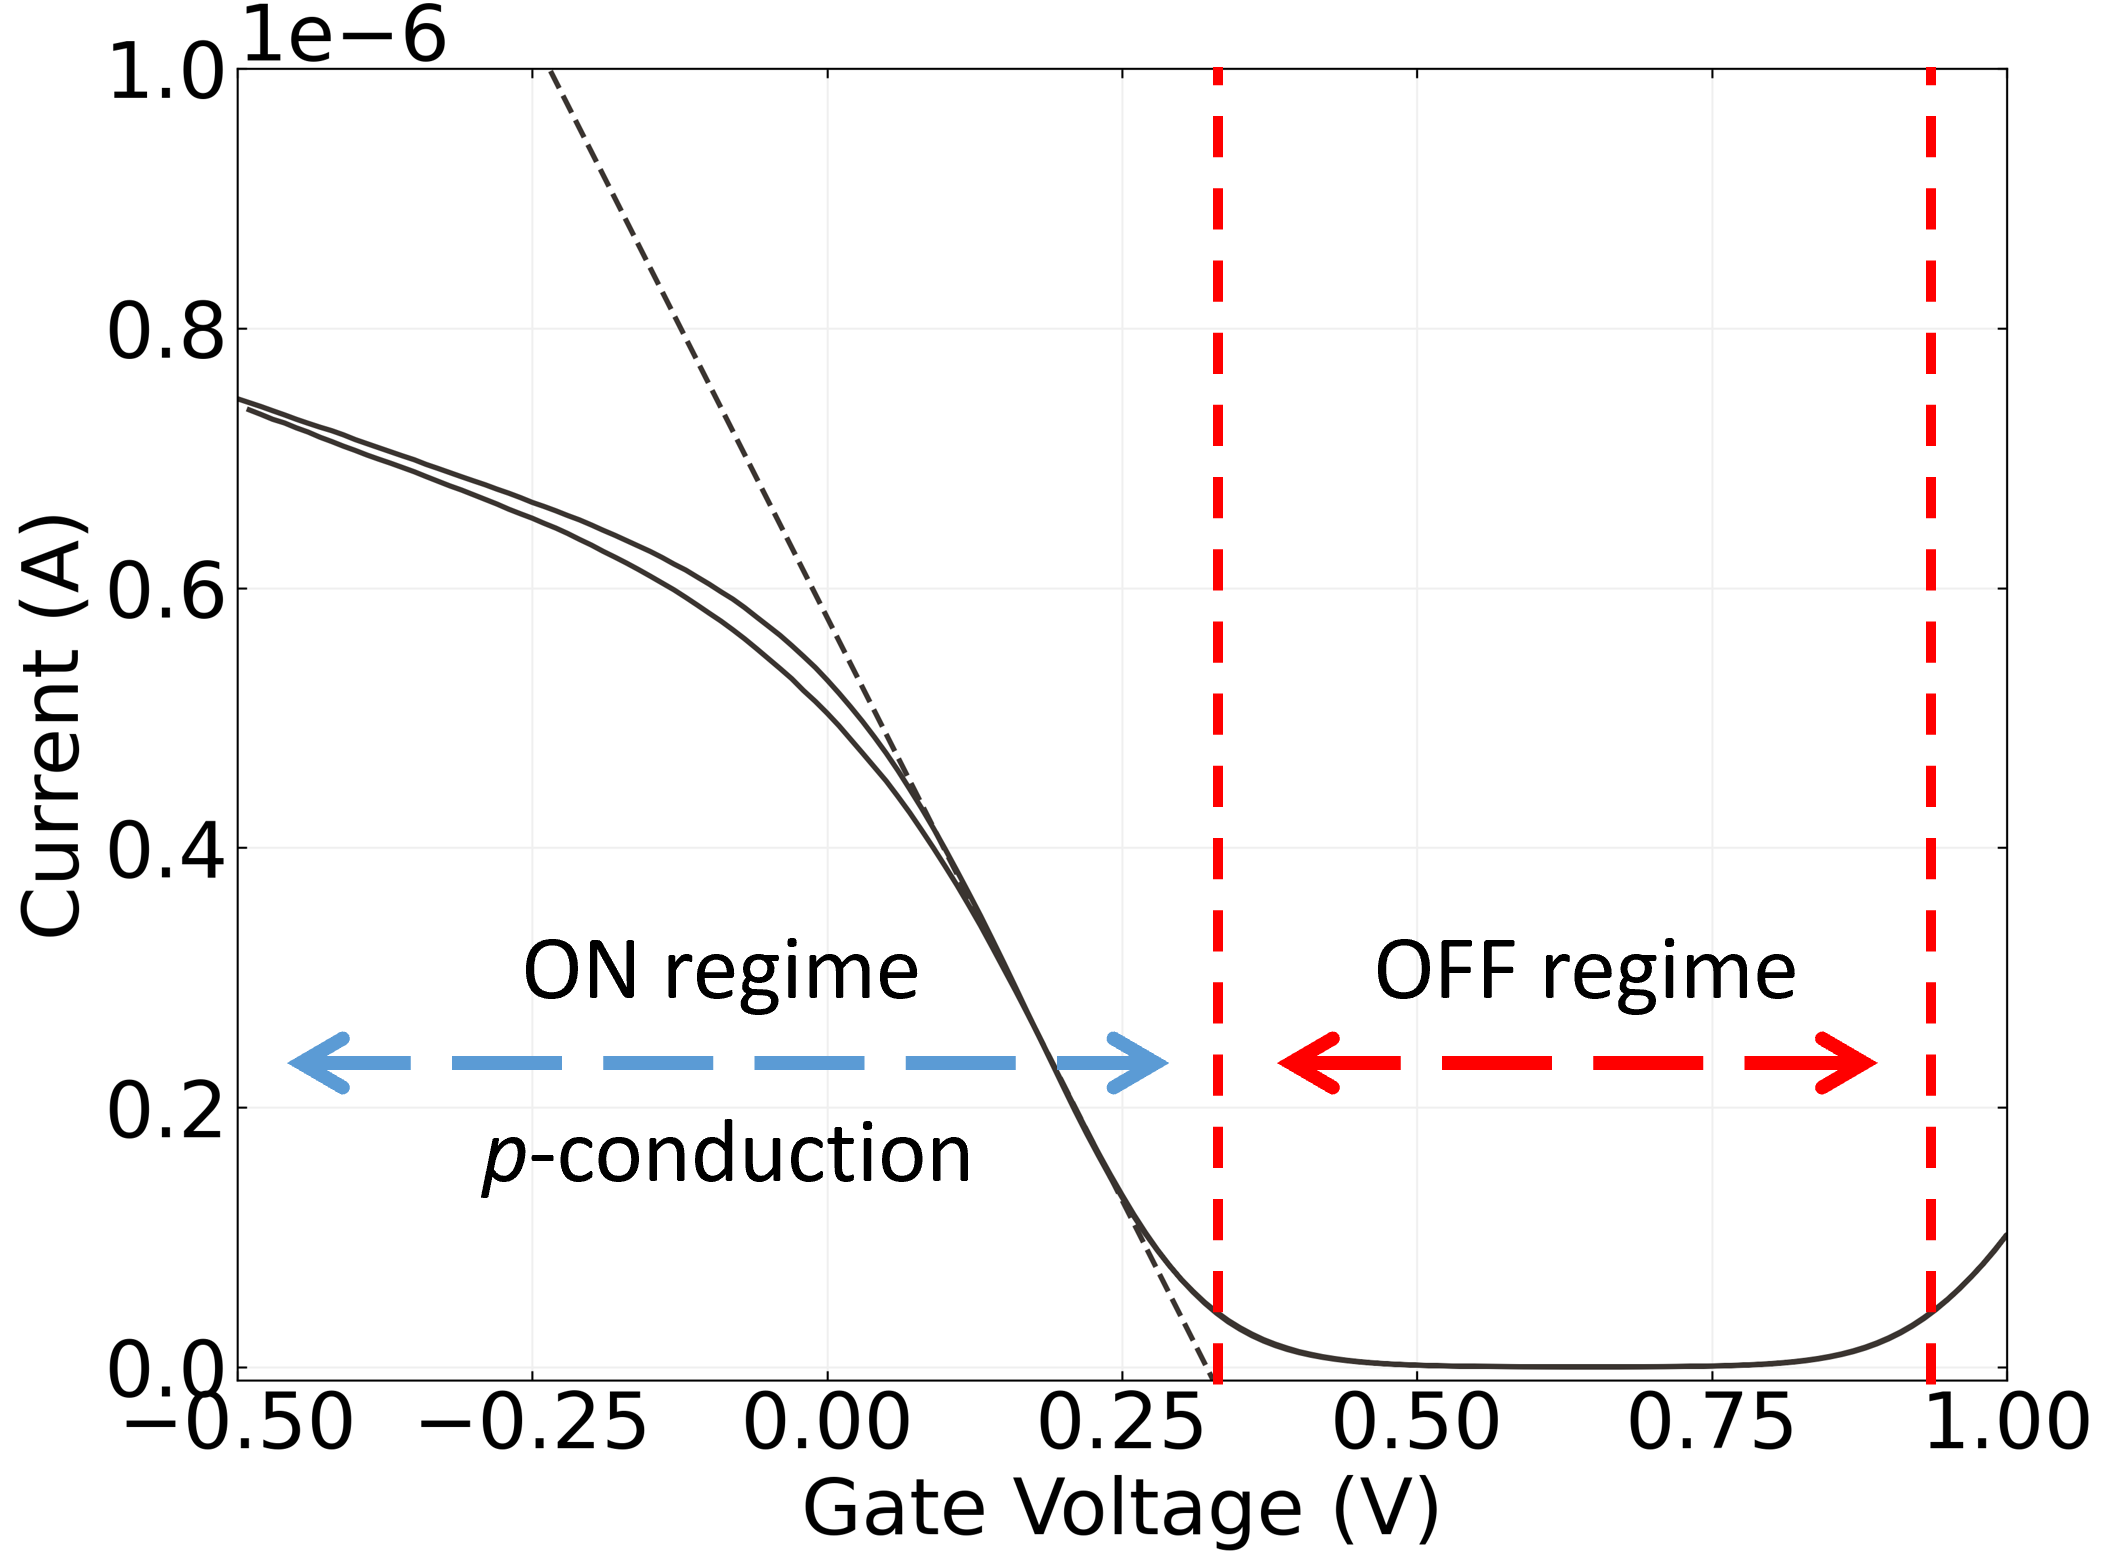
\includegraphics{figures/ch2/CNT_transfer_2.png}

}

}

\end{minipage}%
%
\begin{minipage}[t]{0.01\linewidth}

{\centering 

~

}

\end{minipage}%

\caption{\label{fig-CNT-characteristics}Liquid-gated transfer
characteristics of a single carbon nanotube network field-effect
transistor channel, using a logarithmic scale in (a) and using a linear
scale in (b) to emphasise different features of the same dataset. The
subthreshold slope is shown with a black dotted line, while the
threshold voltages are shown with red dotted lines. The ON and OFF
regimes are also indicated on both figures.}

\end{figure}

Like graphene transistors, mixed-chirality carbon nanotube transistors
are naturally ambipolar: they can conduct both electrons and holes.
Holes travel at highly negative voltages, while electrons travel at
highly positive voltages. At intermediary voltages, both electrons and
holes flow \autocite{Yao2021}. Transistor behaviour can be made unipolar
through doping the semiconducting carbon nanotubes or by choosing an
electrode metal with a particularly high work function, increasing the
Schottky barrier for one type of charge
\autocite{Avouris2007,Cao2009,Yao2021}. For example, the use of gold
electrodes promotes \(p\)-type behaviour over \(n\)-type behaviour due
to the work function of the metal; ambient adsorption of oxygen will
weakly dope the semiconducting carbon nanotubes and likewise promote
\(p\)-type behaviour \autocite{McEuen2002,Cao2009,Shkodra2021}.

In a unipolar transistor, the threshold voltage \(V_t\) is equal to the
gate voltage required to prevent charge carriers flowing across the
channel \autocite{Petti2016,Shkodra2021}. The size of the Schottky
barriers, and therefore current flow, can be controlled by altering the
Fermi energy of the semiconducting nanotubes using the applied gate
voltage \(V_g\) \autocite{Nakanishi2002,Avouris2007,Heller2008}. In
ambipolar devices, two separate threshold voltages exist for each type
of charge carrier, \(V_{t,h}\) and \(V_{t,e}\)
\autocite{Reiner-Rozman2015}. In the region between these gate voltages,
both holes and electrons flow through the channel. If percolating
pathways consisting entirely of m-CNTs are present, the off current
\(I_{off}\) flows through these pathways, as conduction through metallic
nanotubes is largely unaffected by changes in \(V_g\)
\autocite{Fuhrer2000,Topinka2009}. If there are no unblocked m-CNT
pathways, \(I_{off}\) is entirely due to Schottky barrier tunnelling
\autocite{Avouris2007}. \(V_t\) can be estimated by extrapolating the
trendline of the linear region of the transfer characteristics to the
\(V_g\) axis. The intercept \(V_{gInt}\) is approximately equal to the
threshold voltage when \(V_{ds}\) is close to zero
\autocite{Petti2016,Li2023}. This is only a rough estimate of the actual
device \(V_t\), but is sufficient for comparing the gating behaviour of
different devices \autocite{Li2023}.

Various other device parameters can be extracted which reflect the
morphology of the carbon nanotube network. Partial alignment of a
random-network carbon nanotube network maximises the transconductance of
a device, as this creates more semiconducting pathways, increasing
current while preserving the presence of gateable junctions within the
network \autocite{Cao2009,Rouhi2010,Rouhi2011a,Jang2015,Li2023}. The
on-off ratio of a carbon nanotube device is largely decided by the ratio
of s-CNTs to m-CNTs. The relative proportion of metallic carbon
nanotubes in the network determines the size of \(I_{off}\). Therefore,
unlike a graphene device, the off current can be readily reduced by
eliminating percolating metallic pathways for increased
\(I_{on}/I_{off}\) \autocite{Hu2004,Cao2009,Rouhi2010,Rouhi2011a}. In a
liquid-gated environment, the gate leakage current of a sparse carbon
nanotube transistor can approach \(I_d\), leading to significant device
noise. A dense network or a graphene device can therefore give enhanced
signal-to-noise ratio during sensing \autocite{Ohno2015}. Noyce \emph{et
al.} found that fully-on back-gated carbon nanotube devices typically
exhibit a \(\sim\) 3 hour period of steep signal drift, followed by
steady-state current flow. This settling behaviour was found to be
reversible and highly characteristic of a particular channel, and could
be modelled using a sum of three exponentials \autocite{Noyce2019}.

Threshold Voltage: minimum gate-to-source voltage that is needed to
create a conducting path between the electrodes

Quantative measurement of leftward shift in transfer curve Use minima of
curve in reverse sweep direction (more consistent than reading in
forward sweep direction) I compared the transfer characteristics after
then rinse steps to the pristine characteristics Transfer shifts where
current drops to zero are excluded (indicates delamination/damage to
channel)

Second quantative measurement of leftward shift in transfer curve Use
curve in reverse sweep direction (more consistent than reading in
forward sweep direction) Separate readings for left and right hand sides
of transfer curve (left side = electrons dominant carrier, right side =
holes dominant carrier) Transfer shifts where current drops to zero are
excluded (indicates delamination/damage to channel) This gives us a
quantitative idea of whether the transfer shifts in slides 5/6 are
stable (remain the same/similar after rinse steps)

\hypertarget{sec-CNT-sensing-mechanisms}{%
\subsection{Sensing Behaviour}\label{sec-CNT-sensing-mechanisms}}

As all atoms are at the surface of the carbon nanotube structure,
nanotubes are very sensitive to their surroundings and therefore
suitable for sensing use \autocite{Cao2009,Yao2021,Shkodra2021}. The
chirality and diameter of a carbon nanotube affects both its coupling
with the gate and its surface chemistry, which determines the sensing
mechanisms available to a single CNT. Only s-CNTs can be
electrostatically gated; m-CNTs and larger diameter nanotubes are
typically more reactive \autocite{Cao2009,Li2023}; and the nanotube
chirality (\(n,m\)) can determine the strength of binding to DNA in a
base sequence-dependent manner \autocite{Rouhi2011a}. Carbon nanotubes
have been used for vapour-phase sensing since 2000, when Kong \emph{et
al.} found that the resistance over a single CNT channel was modified
when exposed to gas molecules like NO\(_2\) and NH\(_3\)
\autocite{Kong2000}. In a range of gas sensor applications, carbon
nanotubes can detect the presence of analyte down to the parts per
billion level \autocite{Chen2019,Yao2021}. However, in general, device
specificity of response is low, where nanotubes respond to many
different analytes in a similar manner. To enhance specificity, surface
functionalisation is often performed using either inorganic or
biological materials, such as enzymes, antibodies, aptamers and proteins
\autocite{Cao2009,Shkodra2021,Yao2021}.

For carbon nanotube network transistors, sensing mechanisms include
electrostatic gating, charge transfer, Schottky barrier modulation,
capacitance modulation and charge scattering. Response mechanisms may
take place at the gate, the junctions between channel and contact, or at
the semiconductor channel
\autocite{Heller2008,Battie2011,Boyd2014,Tran2016,Li2023}. Modification
of the channel-metal Schottky barrier can dominate sensing activity, and
this can complicate the identification of mechanisms underlying the
sensing behaviour \autocite{Cao2009,Boyd2014,Schroeder2019}. The
encapsulation layer shown in Figure~\ref{fig-gating-schematics} is added
to separate the electrodes from the channel-metal junction and prevent
these responses \autocite{Heller2008,Shkodra2021}. If there are few
Schottky barriers present in the network of an encapsulated device, the
predominant sensing mechanism is either charge transfer from the analyte
to channel \autocite{Allen2007,Battie2011} or electrostatic gating
\autocite{Heller2008}. The charge transfer mechanism involves direct
addition of charge carriers to the channel, while the gating mechanism
results from a nearby charge inducing an opposite polarity charge in the
channel. Both changes alter the relationship between \(V_g\) and \(I_d\)
and shift the carrier threshold voltages
\autocite{Tran2016,Shkodra2021}. However, when Schottky and other
potential barriers are frequent, barrier modulation may make a
significant contribution to sensing responses
\autocite{Boyd2014,Murugathas2019a}.

\cleardoublepage
\phantomsection
\addcontentsline{toc}{part}{Appendices}
\appendix

\hypertarget{sec-vapour-sensor-components}{%
\chapter{Vapour System Hardware}\label{sec-vapour-sensor-components}}

\hypertarget{tbl-vapour-sensor-components}{}
\begin{longtable}[t]{>{\raggedright\arraybackslash}p{5.5cm}>{\raggedright\arraybackslash}p{4.5cm}>{\raggedright\arraybackslash}p{3.75cm}}
\caption{\label{tbl-vapour-sensor-components}Major components used in construction of the vapour delivery system
described in this thesis. }\tabularnewline

\toprule
Description & Part No. & Manufacturer\\
\midrule
Mass flow controller, 20 sccm full scale & GE50A013201SBV020 & MKS Instruments\\
Mass flow controller, 200 sccm full scale & GE50A013202SBV020 & MKS Instruments\\
Mass flow controller, 500 sccm full scale & FC-2901V & Tylan\\
Analogue flowmeter, 240 sccm max. flow & 116261-30 & Dwyer\\
Micro diaphragm pump & P200-B3C5V-35000 & Xavitech\\
\addlinespace
Analogue flow controller, for micro diaphragm pump & X3000450 & Xavitech\\
10 mL Schott bottle & 218010802 & Duran\\
PTFE connection cap system & Z742273 & Duran\\
Baseline VOC-TRAQ flow cell, red & 043-951 & Mocon\\
Humidity and temperature sensor & T9602 & Telaire\\
\addlinespace
Enclosure, for humidity and temperature sensor & MC001189 & Multicomp Pro\\
\bottomrule
\end{longtable}

\hypertarget{sec-python}{%
\chapter{Python Code for Data Analysis}\label{sec-python}}

\hypertarget{code-repository}{%
\section{Code Repository}\label{code-repository}}

The code used for general analysis of field-effect transistor devices in
this thesis was written with Python 3.8.8. Contributors to the code used
include Erica Cassie, Erica Happe, Marissa Dierkes and Leo Browning. The
code is located on GitHub and the research group OneDrive, and is
available on request.

\hypertarget{sec-histogram-analysis}{%
\section{Atomic Force Microscope Histogram
Analysis}\label{sec-histogram-analysis}}

The purpose of this code is to analyse atomic force microscope (AFM)
images of carbon nanotube networks in .xyz format taken using an atomic
force microscope and processed in Gwyddion (see
\textbf{?@sec-afm-characterisation}). It was originally designed by
Erica Happe in Matlab, and adapted by Marissa Dierkes and myself for use
in Python. The code imports the .xyz data and sorts it into bins 0.15 nm
in size for processing. To perform skew-normal distribution fits, both
\emph{scipy.optimize.curve\_fit} and \emph{scipy.stats.skewnorm} modules
are used in this code.

\hypertarget{sec-raman-analysis}{%
\section{Raman Spectroscopy Analysis}\label{sec-raman-analysis}}

The purpose of this code is to analyse a series of Raman spectra taken
at different points on a single film (see
\textbf{?@sec-raman-characterisation}). Data is imported in a series of
tab-delimited text files, with the low wavenumber spectrum (100
cm\(^{-1} - 650\) cm\(^{-1}\)) and high wavenumber spectrum (1300
cm\(^{-1} - 1650\) cm\(^{-1}\)) imported in separate datafiles for each
scan location.

\hypertarget{sec-field-effect-transistor-analysis}{%
\section{Field-Effect Transistor
Analysis}\label{sec-field-effect-transistor-analysis}}

The purpose of this code is to analyse electrical measurements taken of
field-effect transistor (FET) devices. Electrical measurements were
either taken from the Keysight 4156C Semiconductor Parameter Analyser,
National Instruments NI-PXIe or Keysight B1500A Semiconductor Device
Analyser as discussed in \textbf{?@sec-electrical-characterisation}; the
code is able to analyse data in .csv format taken from all three
measurement setups. The main Python file in the code base consists of
three related but independent modules: the first analyses and plots
sensing data from the FET devices, the second analyses and plots
transfer characteristics from channels across a device, and the third
compares individual channel characteristics before and after a
modification or after each of several modifications. The code base also
features a separate config file and style sheet which govern the
behaviour of the main code. The code base was designed collaboratively
by myself and Erica Cassie over GitHub using the Sourcetree Git GUI.


\backmatter
\printbibliography


\end{document}
